\documentclass[12pt, letterpaper, oneside]{report}

% =============================================================================
% PREÁMBULO GLOBAL - CONFIGURACIÓN PROFESIONAL
% =============================================================================

% --- CODIFICACIÓN E IDIOMA ---
\usepackage[utf8]{inputenc}
\usepackage[T1]{fontenc}
\usepackage[spanish, es-tabla, es-nodecimaldot]{babel} % es-nodecimaldot para que no cambie el punto por coma en matemáticas si se desea

% --- TIPOGRAFÍA PROFESIONAL ---
\usepackage{mathptmx}       % Times para texto y matemáticas
\usepackage[scaled=0.92]{helvet} % Helvetica para sans-serif
\usepackage{courier}        % Courier para monoespaciado

% Mejoras tipográficas avanzadas
\usepackage{microtype}
\usepackage{textcomp}

% --- FORMATO DE PÁGINA PROFESIONAL ---
\usepackage{geometry}
\geometry{
	left=3cm,
	right=2.5cm,
	top=2.5cm,
	bottom=2.5cm,
	headheight=15pt
}

\usepackage{setspace}
\onehalfspacing

% Encabezados y pies de página
\usepackage{fancyhdr}
\pagestyle{fancy}
\fancyhf{}
\fancyhead[R]{\nouppercase{\leftmark}}
\fancyfoot[C]{\thepage}
\renewcommand{\headrulewidth}{0.5pt}
\renewcommand{\footrulewidth}{0pt}

\fancypagestyle{plain}{
	\fancyhf{}
	\fancyfoot[C]{\thepage}
	\renewcommand{\headrulewidth}{0pt}
}

% --- MATEMÁTICAS Y SÍMBOLOS ---
\usepackage{amsmath}
\usepackage{amssymb}
\usepackage{amsthm}
\usepackage{mathtools}
\usepackage{csquotes}

% --- GRÁFICOS Y TABLAS ---
\usepackage{graphicx}
\usepackage{float}
\usepackage{booktabs}
\usepackage{multirow}
\usepackage{makecell}
\usepackage{subcaption}
\usepackage{caption}

\captionsetup{
	font=small,
	labelfont=bf,
	format=plain,
	justification=centering,
	singlelinecheck=false
}

% --- COLORES ---
\usepackage{xcolor}
\definecolor{darkblue}{RGB}{0,51,102}
\definecolor{darkred}{RGB}{139,0,0}

% --- DIAGRAMAS Y ALGORITMOS ---
\usepackage{tikz}
\usetikzlibrary{shapes.geometric, arrows, positioning, calc, shadows}
\usepackage{algorithm}
\usepackage{algpseudocode}

\floatname{algorithm}{Algoritmo}
\renewcommand{\algorithmicrequire}{\textbf{Entrada:}}
\renewcommand{\algorithmicensure}{\textbf{Salida:}}

% --- LISTADOS DE CÓDIGO ---
\usepackage{listings}
\lstset{
	basicstyle=\ttfamily\small,
	keywordstyle=\color{darkblue}\bfseries,
	commentstyle=\color{gray}\itshape,
	stringstyle=\color{darkred},
	numbers=left,
	numberstyle=\tiny\color{gray},
	stepnumber=1,
	numbersep=8pt,
	showstringspaces=false,
	breaklines=true,
	frame=single,
	backgroundcolor=\color{white},
	captionpos=b,
	inputencoding=utf8,
	extendedchars=true,
	literate={á}{{\'a}}1 {é}{{\'e}}1 {í}{{\'i}}1 {ó}{{\'o}}1 {ú}{{\'u}}1 {ñ}{{\~n}}1 % Soporte para tildes en código
}

% --- BIBLIOGRAFÍA (BIBLATEX CON BIBER) ---
\usepackage[
style=ieee,
backend=biber,
sorting=none,
maxbibnames=99,
giveninits=true,
doi=true,
url=true,
eprint=false
]{biblatex}

% Archivo de bibliografía (asegúrate de tener este archivo en la carpeta)
\addbibresource{referencias.bib}

% --- ENLACES (Hyperref debe cargarse casi al final) ---
\usepackage[hidelinks]{hyperref}
\hypersetup{
	colorlinks=true,
	linkcolor=black,
	citecolor=darkblue,
	urlcolor=darkblue,
	pdfborder={0 0 0},
	pdftitle={Sistema de Seguimiento Ocular},
	pdfauthor={Tu Nombre},
	pdfsubject={Tesis de Física},
	pdfkeywords={Eye Tracking, Biometría, Visión por Computadora}
}

% --- AJUSTES FINOS ---
\widowpenalty=10000
\clubpenalty=10000

% --- FORMATO DE CAPÍTULOS (Titlesec después de hyperref) ---
\usepackage{titlesec}
\titleformat{\chapter}[display]
{\normalfont\huge\bfseries}
{\chaptertitlename\ \thechapter}
{20pt}
{\Huge}
\titlespacing*{\chapter}{0pt}{-20pt}{40pt}

% --- UNIDADES FÍSICAS ---
\usepackage{siunitx}
\sisetup{
	detect-all, % Nota: En versiones muy nuevas de siunitx esto puede generar warning, pero compila.
	output-decimal-marker = {,},
	group-separator = {.},
	group-minimum-digits = 4
}

% =============================================================================
% CUERPO DEL DOCUMENTO
% =============================================================================
\begin{document}
	
	% --- PRELIMINARES (Numeración Romana) ---
	\pagestyle{empty}
	\pagenumbering{roman}
	
	% Portada
	% =============================================================================
% PORTADA COMPACTA UNA SOLA PÁGINA - DISPOSICIÓN HORIZONTAL
% =============================================================================

\begin{titlepage}
	\begin{center}
		
		\vspace*{0.3cm}
		
		% --- LOGO ---
		\includegraphics[width=0.14\textwidth]{Imagenes/logo_ULA.png}
		
		\vspace{0.2cm}
		
		% --- ENCABEZADO INSTITUCIONAL ---
		{\normalsize\bfseries
			UNIVERSIDAD DE LOS ANDES\\[0.15cm]
		}
		
		{\small
			FACULTAD DE CIENCIAS\\[0.08cm]
			DEPARTAMENTO DE FÍSICA\\[0.08cm]
			MÉRIDA -- VENEZUELA
		}
		
		\vspace{0.8cm}
		
		% --- TÍTULO ---
		{\Large\bfseries
			ESTUDIO DE UN SISTEMA DE SEGUIMIENTO OCULAR\\[0.25cm]
			BASADO EN TÉCNICAS DE\\[0.25cm]
			PROCESAMIENTO DE IMÁGENES
		}
		
		\vspace{0.3cm}
		
		{\normalsize
			Una Propuesta Experimental
		}
		
		\vspace{0.8cm}
		
		% --- DESCRIPCIÓN DEL TRABAJO ---
		{\small
			Trabajo Especial de Grado presentado\\
			como requisito parcial para optar al título de\\[0.2cm]
			\textbf{LICENCIADO EN FÍSICA}
		}
		
		\vspace{2.2cm}  % Más espacio para bajar los nombres
		
		% --- AUTOR, TUTOR Y JURADOS EN DISPOSICIÓN HORIZONTAL ---
		\noindent
		\begin{minipage}[t]{0.48\textwidth}
			\raggedright
			\normalsize
			\textbf{Autor:}\\
			Víctor Toro\\
			\vspace{0.4cm}
			
			\textbf{Tutor Académico:}\\
			Prof. Juan Carlos Villegas
		\end{minipage}
		\hfill
		\begin{minipage}[t]{0.48\textwidth}
			\raggedleft
			\normalsize
			\textbf{Jurados:}\\
			Dr. John Ferreira\\
			Profa. Stephanie Carrillo
		\end{minipage}
		
		\vspace{1.8cm}  % Espacio reducido entre nombres y fecha
		
		% --- FECHA ---
		{\normalsize
			MÉRIDA, ENERO DE 2026
		}
		
		\vspace{0.5cm}
		
	\end{center}
\end{titlepage}
	
	% Dedicatoria y Agradecimientos
	% No lleva título de capítulo visible, suele ser una página "muda" con el texto.

\vspace*{6cm} % Espacio vertical para bajar el texto

\begin{flushright}
    \begin{minipage}{0.6\textwidth}
        \begin{flushright}
            \itshape % Texto en cursiva
            A mis padres, por ser el pilar fundamental de mi vida y por su apoyo incondicional en cada paso de este camino.
            
            \vspace{0.5cm}
            
            A Dios, por la fortaleza espiritual.
            
            \vspace{0.5cm}
            
            A mí mismo, por la perseverancia y la resiliencia demostrada para alcanzar esta meta.
        \end{flushright}
    \end{minipage}
\end{flushright}

\vfill % Empuja todo lo anterior hacia arriba si sobra espacio
	\chapter*{Agradecimientos} % El * hace que no lleve número (Capítulo X)
\addcontentsline{toc}{chapter}{Agradecimientos} % Pero lo agregamos al índice manual

Quiero expresar mi más sincero agradecimiento a todas las personas e instituciones que hicieron posible la realización de este Trabajo Especial de Grado.

En primer lugar, a la Universidad de Los Andes y al Departamento de Física, mi casa de estudios, por haberme brindado la formación académica y las herramientas necesarias para mi desarrollo profesional.

A mi tutor, Prof. Juan Carlos Villegas, por su invaluable guía, paciencia y conocimientos compartidos durante todo el proceso de investigación. Gracias por confiar en esta propuesta y por sus acertadas correcciones que enriquecieron sustancialmente este trabajo.

A la Profa. Stephanie Carrillo, por su apoyo constante, sus consejos académicos y su disposición para colaborar en la revisión de los avances de esta tesis.

A mis padres y familiares, por su amor, sacrificio y comprensión durante mis años de estudio. Este logro es también suyo.

A mis compañeros y amigos de la carrera, con quienes compartí largas horas de estudio, retos y alegrías. Gracias por hacer el camino más llevadero.

Finalmente, a todos aquellos que de una u otra forma contribuyeron con un granito de arena para culminar esta etapa de mi vida.

\vspace{2cm}

\begin{flushright}
    \textbf{Víctor Toro}
\end{flushright}
	
	% =========================================================================
	% RESUMEN 
	% =========================================================================
	\chapter*{Resumen}
\addcontentsline{toc}{chapter}{Resumen}

El ojo es una fuente de información valiosa que, al ser analizada rigurosamente, permite no solo obtener resultados biométricos únicos, sino también aplicar estos hallazgos en áreas diversas. Bajo esta premisa, esta investigación desarrolló un sistema de seguimiento ocular de bajo costo capaz de identificar personas y controlar interfaces mediante la mirada.

La metodología empleó un enfoque híbrido que combina características físicas con patrones dinámicos de movimiento (velocidad y precisión). Las pruebas con 15 participantes arrojaron una exactitud de identificación del 83.5\%, superando a los métodos que solo utilizan imágenes estáticas. Como aplicación práctica, se validó la viabilidad técnica del sistema para el control de cursor en tecnologías asistivas.

Adicionalmente, el análisis reveló que los patrones oculares varían según el nivel de cansancio e iluminación, sugiriendo un nuevo uso potencial para el monitoreo de fatiga en salud ocupacional. En conclusión, este trabajo demuestra que es factible implementar soluciones avanzadas de biometría y accesibilidad sin depender de hardware costoso.

\vspace{0.5cm}

\textbf{Palabras clave:} Seguimiento ocular, biometría, procesamiento de imágenes, tecnologías asistivas, inteligencia artificial.

	
	% Activar numeración de páginas para índices
	\pagestyle{plain}
	
	% Índices
	\tableofcontents
	\clearpage
	
	\listoffigures
	\addcontentsline{toc}{chapter}{Lista de Figuras}
	\clearpage
	
	\listoftables
	\addcontentsline{toc}{chapter}{Lista de Tablas}
	\clearpage
	
	% Introducción (sin numeración de capítulo, pero en TOC)
	\chapter*{Introducción}
\addcontentsline{toc}{chapter}{Introducción}

El análisis del movimiento ocular permite comprender aspectos fundamentales de la fisiología humana y desarrollar nuevas interfaces tecnológicas. El ojo proporciona información biológica y cinemática única: el patrón del iris y la pupila constituyen identificadores morfológicos robustos, mientras que las trayectorias oculares permiten inferir estados neurológicos y patrones de comportamiento \textcite{komogortsev2010}.

El desarrollo científico en este campo se ha visto limitado por la barrera económica de los dispositivos comerciales de seguimiento ocular (\textit{eye-trackers}), cuyos costos restringen su aplicación masiva. Esta investigación desarrolla un sistema integral de seguimiento ocular de bajo costo fundamentado en técnicas de procesamiento de imágenes y visión artificial.

El objetivo es doble: validar la viabilidad de la biometría oculomotora para identificación de individuos y evaluar su aplicabilidad como interfaz de control humano-máquina. Se diseñó un sistema de captura basado en sensores CMOS operando a 120 FPS en el espectro infrarrojo cercano (NIR), permitiendo la reconstrucción de la dinámica ocular con alta fidelidad temporal.

La metodología integra principios de óptica geométrica con algoritmos de aprendizaje profundo. Se implementó una arquitectura basada en la red neuronal YOLOv8 para la detección de la pupila, complementada con filtros Savitzky-Golay para el cálculo de derivadas cinemáticas (velocidad, aceleración y \textit{Jerk}). A diferencia de los sistemas biométricos estáticos tradicionales, esta investigación utiliza una huella oculomotora dinámica, demostrando que la interacción entre anatomía ocular y micro-estrategia de movimiento es única para cada sujeto.

Los resultados experimentales, obtenidos de 15 participantes, validan el cumplimiento de leyes fisiológicas fundamentales como la \textit{Main Sequence} \textcite{bahill1975} ($R^2 > 0.90$), y demuestran una exactitud de clasificación biométrica del 83.5\% mediante \textit{Random Forest} \textcite{breiman2001}. Asimismo, se presenta una prueba de concepto para control de cursor mediante la mirada, estableciendo las bases para tecnologías asistivas accesibles.
	
	% --- CONTENIDO PRINCIPAL (Numeración Arábiga) ---
	\clearpage
	\pagenumbering{arabic} % Reinicia contador a 1
	\pagestyle{fancy}
	
	% Capítulos
	% --- CAPÍTULO I ---
\chapter{Planteamiento del Problema}

\section{El problema}

Esta investigación se fundamenta en la premisa de que el ojo proporciona información biológica y cinemática única. Morfológicamente, el patrón del iris y las dimensiones de la pupila actúan como identificadores biométricos robustos e irrepetibles. Dinámicamente, el análisis de los movimientos oculares, tales como vibraciones o anomalías en la trayectoria, permite inferir datos significativos sobre el estado fisiológico y neurológico del individuo.

Un aspecto tecnológicamente relevante de este campo es la capacidad de traducir la mirada en comandos de control para la interacción humano-máquina. Estas aplicaciones son críticas en medicina, ofreciendo soluciones de asistencia para personas con movilidad reducida, y en áreas como la neurociencia, interesadas en modelar el comportamiento humano.

El objetivo central es implementar un sistema integral de captura y procesamiento de patrones oculares. El sistema permitirá validar la identificación biométrica y abrir la posibilidad a la creación de herramientas de control por mirada que mejoren la calidad de vida de usuarios con discapacidades motoras.

Díaz y Rojas \cite{diaz2021} sostienen que:

\begin{quote}
	El sentido más importante que proporciona la mayor cantidad de información, es el sentido de la vista y por esto, el estudio de la actividad visual mediante la técnica del seguimiento ocular (eye-tracking), se ha convertido en un tema de interés durante los últimos años, para las investigaciones en educación matemática, que incorporan los avances de la neurociencia cognitiva (p. 39).
\end{quote}

La cita hace alusión especial a la educación en matemática, ya que las investigadoras utilizan el seguimiento ocular para comprender cómo los estudiantes procesan la lectura de problemas. El seguimiento ocular está siendo estudiado en todas las áreas del conocimiento.

La física proporciona herramientas para abordar y resolver problemas prácticos y actuales. Su capacidad para modelar, analizar y comprender fenómenos naturales permite el desarrollo de soluciones que trascienden teorías abstractas y encuentran aplicaciones directas para mejorar la vida de las personas.

Se plantean cuatro interrogantes que guiarán esta investigación:

\begin{enumerate}
	\item ¿Cómo implementar un sistema de captura de imágenes o videos del ojo?
	\item ¿De qué manera se pueden analizar los datos recolectados mediante técnicas de procesamiento de imágenes?
	\item ¿Cómo identificar patrones de movimiento ocular a partir de los datos obtenidos?
	\item ¿Cómo se puede evaluar el sistema para su aplicación en el control de un cursor?
\end{enumerate}

\section{Objetivos}

Esta investigación se estructura mediante objetivos específicos. Como indican Ramírez et al. \cite{ramirez2004}: ``los objetivos nos permiten dejar en claro cuál va a ser el alcance de nuestro trabajo de investigación, nos indican el punto de llegada, lo que queremos lograr'' (p. 56).

Se establece un objetivo general y cuatro objetivos específicos.

\subsection{Objetivo general}
Implementar un sistema de seguimiento ocular a partir de técnicas de procesamiento de imágenes para el análisis de patrones oculares.

\subsection{Objetivos específicos}
\begin{enumerate}
	\item Implementar un sistema de captura de imágenes o videos del ojo.
	\item Analizar los datos recolectados mediante técnicas de procesamiento de imágenes.
	\item Identificar patrones de movimiento ocular a partir de los datos obtenidos.
	\item Evaluar el sistema para su posible aplicación en el control de un cursor.
\end{enumerate}

\section{Justificación}

Esta investigación integra conocimientos de física y herramientas tecnológicas para abordar problemas reales en el campo de la asistencia médica y la interacción humano-máquina. Los principios de la física, especialmente en áreas como la óptica y el análisis computacional, se vinculan con la medicina para desarrollar alternativas que mejoren la calidad de vida.

El seguimiento ocular permite la comunicación sin necesidad de movimientos físicos o habla, lo que resulta especialmente útil para personas con discapacidades motoras derivadas de lesiones cerebrales, parálisis cerebral o accidentes cerebrovasculares.

La identificación de patrones de movimiento ocular permite desarrollar herramientas asistivas y aporta al avance interdisciplinario de la física aplicada, la tecnología y la medicina.

Como señala Arias \cite{arias2010}, en esta sección de la justificación ``deben señalarse las razones por las cuales se realiza la investigación y sus posibles aportes desde el punto de vista teórico o práctico'' (p. 105).

El análisis de imágenes permite observar fenómenos invisibles a simple vista, impulsando avances tecnológicos y científicos que mejoran la calidad de vida.

\section{Organización de la tesis}

Este trabajo se encuentra estructurado en cinco capítulos:

\begin{description}
	\item[Capítulo 1: El problema a estudiar.] Se plantea el problema de investigación, se establecen los objetivos y se justifica la importancia del estudio.
	
	\item[Capítulo 2: Marco teórico.] Se expone una revisión conceptual sobre los temas fundamentales relacionados con el procesamiento de imágenes, la extracción de información a partir de los datos y conceptos fisiológicos relevantes para la investigación, que sirve como sustento para el desarrollo del proyecto.
	
	\item[Capítulo 3: Metodología.] Se describe el enfoque metodológico adoptado, las etapas principales del proceso de recolección y análisis de datos, así como las herramientas y técnicas empleadas para el tratamiento de la información y el desarrollo experimental.
	
	\item[Capítulo 4: Resultados.] Se presentan los resultados obtenidos a partir del análisis de los datos, acompañados de su respectiva interpretación y discusión preliminar.
	
	\item[Capítulo 5: Discusión y conclusiones.] Se realiza una discusión detallada de los resultados en comparación con investigaciones previas, se exponen las conclusiones alcanzadas y se proponen recomendaciones para futuras investigaciones.
\end{description}

Finalmente, se incluyen varios anexos que complementan el trabajo, tales como programas utilizados, abreviaturas, glosario de términos y documentación técnica relevante.
	% --- CAPÍTULO II ---
\chapter{Marco Teórico}

% ===================================================================
% 2.1 ANTECEDENTES
% ===================================================================
\section{Antecedentes teóricos de la investigación}

El seguimiento ocular es una técnica que permite registrar y analizar los movimientos de los ojos, proporcionando información valiosa sobre cómo interactúan los individuos con su entorno visual. Esta tecnología ha sido ampliamente utilizada en diversos campos, como la neurociencia, la psicología, la investigación de la experiencia del usuario y el desarrollo de interfaces hombre-máquina.

La física ha contribuido significativamente a este campo, aportando métodos cuantitativos para el análisis del movimiento ocular. Otras áreas del conocimiento también han desarrollado interés por comprender el fenómeno del movimiento ocular y su aplicación en el desarrollo científico.

A continuación se presentan diversos artículos que constituyen la base teórica de la presente investigación. Estos trabajos sustentan la metodología empleada y las técnicas aplicadas.

\subsection{Eye Aspect Ratio (EAR) para Detección de Somnolencia}

El trabajo de Dewi et al. \cite{dewi2022eye} presenta un método innovador para detectar la somnolencia en conductores en tiempo real, basándose en la métrica conocida como Relación de Aspecto del Ojo (EAR), propuesta originalmente por Soukupová y Čech \cite{soukupova2016real}.

Este estudio de Soukupová y Čech es considerado fundamental en la literatura de visión artificial, ya que marcó un cambio de paradigma en el análisis facial: abandonó el procesamiento intensivo de texturas y píxeles en favor de un modelo puramente geométrico basado en puntos de referencia (\textit{landmarks}). Esta abstracción permitió, por primera vez, ejecutar algoritmos de detección de parpadeo con alta precisión en hardware de recursos limitados (como sistemas embebidos), estableciendo el estándar de eficiencia que domina el campo hasta la actualidad.

La técnica se fundamenta en la identificación de 6 puntos de referencia faciales alrededor del contorno ocular. Matemáticamente, el EAR se calcula mediante la relación entre las distancias verticales y la distancia horizontal del ojo, tal como se expresa en la Ecuación \ref{eq:ear_original}:

\begin{equation}
	EAR = \frac{||p_2 - p_6|| + ||p_3 - p_5||}{2 \cdot ||p_1 - p_4||}
	\label{eq:ear_original}
\end{equation}

Donde $p_1$ y $p_4$ corresponden a las comisuras (extremos horizontales), mientras que los pares $(p_2, p_6)$ y $(p_3, p_5)$ representan los puntos del párpado superior e inferior respectivamente. El numerador calcula el promedio de la apertura vertical, y el denominador normaliza esta medida respecto al ancho del ojo, haciendo la métrica invariante a la escala de la imagen y a la distancia del usuario.

En su estudio aplicado, Dewi et al. \cite{dewi2022eye} concluyen que un umbral de EAR de 0.18 ofrece el mejor compromiso entre precisión y rendimiento. Este método tiene un alto potencial para sistemas de seguridad vial en tiempo real, aunque, como se discutirá en el Capítulo 5, la fórmula original presenta limitaciones de estabilidad ante ruido de alta frecuencia que esta tesis busca mitigar mediante una propuesta geométrica densa.

\subsection{Introduction to Eye Tracking: A Hands-On Tutorial}
Gao et al. \cite{gao2025eye_tracking_tutorial} ofrecen una guía accesible sobre los fundamentos del seguimiento ocular. Combina teoría y práctica para facilitar la comprensión de conceptos clave como el funcionamiento de los dispositivos (cámaras infrarrojas), métricas comunes (fijaciones, sacádicos) y su interpretación en contextos como la interacción humano-computadora.

\subsection{Remote Photoplethysmography}
Allado et al. \cite{allado2022remote} evalúan la precisión de la fotopletismografía remota (rPPG) para medir la frecuencia respiratoria de forma no invasiva utilizando cámaras convencionales. La rPPG demostró una correlación significativa con métodos tradicionales, evitando el uso de sensores físicos.

\subsection{AI in Medical Imaging Technology}
Según estudios recientes \cite{ncbi2023ai}, la inteligencia artificial está transformando la imagen médica. Destacan el uso de redes neuronales convolucionales (CNN) y redes generativas antagónicas (GAN) para mejorar la precisión en la detección de anomalías.

\subsection{Abnormal Ocular Movement in Multiple-System Atrophy}
Zhou et al. \cite{zhou2024abnormal} comparan movimientos oculares en pacientes con atrofia multisistémica y enfermedad de Parkinson. Hallaron que las alteraciones en la velocidad y precisión de los sacádicos voluntarios, así como el nistagmo vertical, son marcadores potenciales para el diagnóstico diferencial.

\subsection{Aplicación de la convolución de matrices}
Giménez et al. \cite{gimenez2016aplicacion} abordan la convolución de matrices como herramienta fundamental en el procesamiento de imágenes. Explican cómo los kernels de convolución permiten aplicar filtros (suavizado, detección de bordes) esenciales para las CNN.

\subsection{Analysis of eye-tracking experiments on Tobii T60}
Weigle et al. \cite{weigle2008analysis} analizan el desempeño del dispositivo Tobii T60. Los resultados muestran que proporciona datos útiles para estudios de visualización, aunque su exactitud puede verse afectada por movimientos de cabeza y condiciones ambientales, sugiriendo la necesidad de una calibración cuidadosa.

La revisión bibliográfica expuesta evidencia el vacío existente en soluciones de bajo costo, nicho que esta investigación pretende ocupar, integrando fundamentos matemáticos, principios físicos y avances computacionales.


% ===================================================================
% 2.2 BASES CONCEPTUALES (Anatomía y Movimientos básicos)
% ===================================================================
\section{Bases conceptuales}

\subsection{Anatomía del Ojo Humano}

El ojo es un órgano que permite percibir la luz, convirtiéndola en señales eléctricas que el cerebro interpreta. Es un sentido clave para la supervivencia humana.

\begin{figure}[h]
	\centering
	\includegraphics[width=0.7\textwidth]{Imagenes/ojo.png}
	\caption{Imagen descriptiva del ojo humano.}
	\label{fig:ojo_anatomia}
\end{figure}

Según Cárdenas \cite{cardenas2024}, las partes principales son:

\begin{description}
	\item[Esclera:] Capa más externa del ojo, de color blanco, formada por tejido conectivo denso.
	\item[Córnea:] Capa transparente frontal que ayuda a enfocar la luz.
	\item[Pupila:] Apertura en el centro del iris que regula la entrada de luz.
	\item[Iris:] Estructura de color que controla el tamaño de la pupila mediante músculos.
	\item[Cristalino:] Lente flexible detrás de la pupila que enfoca la luz en la retina.
	\item[Músculos ciliares:] Rodean al cristalino y modifican su grosor para el enfoque.
	\item[Vítreo:] Sustancia gelatinosa que llena el interior del ojo.
	\item[Retina:] Capa sensible a la luz en la parte posterior que contiene fotorreceptores (conos y bastones).
	\item[Nervio óptico:] Transmite la información visual al cerebro.
\end{description}

\subsection{Movimientos oculares básicos}

El sistema oculomotor permite diversos tipos de movimientos, cada uno con funciones específicas \cite{duchowski2017}:

\subsubsection{Fijaciones}
Son períodos durante los cuales el ojo permanece relativamente estático sobre un punto de interés, permitiendo la adquisición de información visual detallada. Típicamente duran entre 200 y 400 ms.

\subsubsection{Sacádicos}
Movimientos rápidos y balísticos que redirigen la fóvea hacia un nuevo objetivo visual. Son los movimientos más veloces del cuerpo humano, alcanzando velocidades de hasta 900°/s.

\subsubsection{Movimientos de seguimiento suave (Smooth Pursuit)}
Permiten al ojo seguir un objeto en movimiento, manteniendo su imagen en la fóvea. Su velocidad máxima es de aproximadamente 30°/s.

\subsection{La secuencia principal (Main Sequence)}

Bahill et al. \cite{bahill1975} establecieron una relación fundamental conocida como la secuencia principal (\textit{Main Sequence}), que describe la relación matemática y determinista entre la amplitud angular de un movimiento sacádico y su velocidad pico. Esta relación modela el comportamiento balístico del ojo mediante la siguiente expresión exponencial:

\begin{equation}
	V_{\text{max}} = V_{\text{sat}} \left(1 - e^{-A/C}\right)
	\label{eq:bahill}
\end{equation}

donde los parámetros tienen la siguiente interpretación física:
\begin{itemize}
	\item $V_{\text{max}}$ es la velocidad pico alcanzada durante el movimiento (en °/s).
	\item $A$ es la amplitud angular total del desplazamiento (en grados).
	\item $V_{\text{sat}}$ es la velocidad de saturación asintótica ($\approx$ 400-800 °/s en adultos sanos). Este valor representa el límite biomecánico máximo de contracción de los músculos extraoculares.
	\item $C$ es la constante de forma ($\approx$ 10°-20°). Este parámetro define la curvatura de la función y delimita la transición entre movimientos pequeños y grandes.
\end{itemize}

Desde el punto de vista dinámico, esta ecuación revela dos regímenes de comportamiento del sistema oculomotor:
\begin{enumerate}
	\item \textbf{Régimen Lineal (para $A \ll C$):} En movimientos pequeños (microsacadas o sacádicos cortos), la velocidad crece proporcionalmente a la distancia. Esto implica que la duración del movimiento se mantiene casi constante.
	\item \textbf{Régimen de Saturación (para $A \gg C$):} A medida que la amplitud aumenta, la velocidad deja de crecer linealmente y se aproxima asintóticamente a $V_{\text{sat}}$. Esto refleja la incapacidad fisiológica de los músculos para acelerar el globo ocular indefinidamente.
\end{enumerate}

Esta ley neurofisiológica es fundamental no solo para describir la cinemática ocular, sino como herramienta de validación de datos: cualquier trayectoria registrada que se desvíe significativamente de esta curva (puntos muy por encima o muy por debajo) puede ser clasificada automáticamente como un artefacto (ruido instrumental, parpadeo) o como una anomalía motora, garantizando así la autenticidad biológica de la señal procesada.

% ===================================================================
% 2.3 SISTEMA DE CAPTURA Y PROCESAMIENTO
% ===================================================================
\section{Sistema de captura y procesamiento}

\subsection{Tecnologías de seguimiento ocular}

Los sistemas de seguimiento ocular (eye trackers) emplean diversas tecnologías para registrar la posición y el movimiento de los ojos. La mayoría de los dispositivos modernos utilizan cámaras que operan en el espectro infrarrojo cercano (NIR), específicamente entre 850 nm y 940 nm, longitudes de onda imperceptibles para el ojo humano pero que permiten una captura eficiente en diferentes condiciones de iluminación.

\subsubsection{Clasificación según el contacto con el usuario}

\begin{description}
	\item[Dispositivos invasivos:] Requieren contacto directo con el ojo, como lentes de contacto con sensores. Ofrecen alta precisión pero son incómodos y no aptos para uso prolongado.
	
	\item[Dispositivos no invasivos:] Basados en video-oculografía (VOG), utilizan cámaras externas para rastrear características del ojo. Son los más comunes en investigación y aplicaciones comerciales por su balance entre precisión y comodidad.
\end{description}

\subsubsection{Configuraciones de captura}

Los sistemas VOG pueden ser:

\begin{itemize}
	\item \textbf{Montados en cabeza (head-mounted):} Cámaras integradas en gafas o cascos, permitiendo movilidad total del usuario. Ideales para estudios en ambientes naturales.
	
	\item \textbf{Remotos (remote):} Cámaras fijas ubicadas frente al usuario, típicamente integradas en monitores. Requieren que el usuario mantenga la cabeza relativamente estable pero ofrecen mayor comodidad para tareas frente a pantallas.
\end{itemize}

\subsection{Fundamentos de la captura por video}

La captura de imágenes del ojo se basa en principios de óptica geométrica y procesamiento digital de señales. Una cámara digital registra la luz reflejada por el ojo a una tasa de muestreo típica de 60 Hz a 1000 Hz, generando secuencias de fotogramas que son procesados en tiempo real o diferido.

\subsubsection{Características de las cámaras}

Para un sistema de seguimiento ocular efectivo, las cámaras deben cumplir con:

\begin{itemize}
	\item \textbf{Resolución espacial:} Mínimo de 640×480 píxeles para capturar detalles de la pupila y reflexiones corneales.
	
	\item \textbf{Tasa de muestreo temporal:} Al menos 60 Hz para capturar movimientos básicos; 250-1000 Hz para análisis de sacádicos de alta velocidad.
	
	\item \textbf{Rango dinámico:} Capacidad de operar bajo diferentes niveles de iluminación ambiente sin saturación.
	
	\item \textbf{Sincronización:} Los sistemas binoculares requieren sincronización precisa entre cámaras para cálculos estereoscópicos.
\end{itemize}

\subsection{Preprocesamiento de la señal}

Las imágenes capturadas requieren una serie de transformaciones para extraer información útil sobre la posición ocular. Este pipeline de procesamiento incluye:

\subsubsection{Conversión a escala de grises}
La mayoría de algoritmos de seguimiento ocular operan sobre imágenes monocromáticas. La conversión se realiza mediante una combinación ponderada de los canales RGB basada en la percepción luminosa humana:
\begin{equation}
	I = 0.2989R + 0.5870G + 0.1140B
\end{equation}
donde $R$, $G$, $B$ son los componentes de color originales.

\subsubsection{Umbralización global}
Permite segmentar regiones de interés aplicando un umbral $T$. La binarización se define como:
\begin{equation}
	I'(x, y) = \begin{cases} 
		255, & \text{si } I(x, y) > T \\
		0, & \text{si } I(x, y) \leq T 
	\end{cases}
\end{equation}
Esto facilita la detección de bordes de la pupila, que típicamente aparece como la región más oscura de la imagen del ojo.

\subsubsection{Filtro de Savitzky-Golay}

Para el preprocesamiento de las señales oculomotoras, se optó por el filtro digital de Savitzky-Golay en lugar de los métodos tradicionales de promedio móvil. Esta técnica realiza un suavizado basado en el ajuste de mínimos cuadrados locales mediante polinomios de bajo grado dentro de una ventana deslizante. Su operación se describe mediante la convolución discreta:

\begin{equation}
	y[i] = \sum_{k=-M}^{M} c_k x[i+k]
\end{equation}

donde $x[i]$ es la señal original, $y[i]$ la señal suavizada, y $c_k$ son los coeficientes de convolución que dependen del orden del polinomio $p$ y del tamaño de la ventana $2M+1$.

La principal ventaja de este enfoque radica en su capacidad para preservar la forma de la onda (\textit{waveform preservation}). A diferencia de los filtros de media móvil, que actúan como filtros paso bajo agresivos y tienden a atenuar la amplitud de los picos (reduciendo artificialmente la velocidad máxima medida) y ensanchar el ancho temporal de los eventos, el filtro Savitzky-Golay mantiene fielmente los momentos estadísticos de orden superior de la señal. Esto resulta crítico para el análisis de movimientos sacádicos, donde la precisión en la detección de la velocidad pico y la aceleración es prioritaria frente a la simple reducción de ruido estocástico.

\subsubsection{Método de la pupila oscura (Dark Pupil)}
Esta técnica utiliza iluminación infrarroja fuera del eje óptico de la cámara (off-axis illumination). La retina absorbe la luz infrarroja, resultando en una pupila que aparece oscura en la imagen, mientras que la esclera y el iris reflejan la luz. Este alto contraste facilita la segmentación automática de la pupila mediante algoritmos de detección de contornos o ajuste de elipses.

\begin{figure}[h]
	\centering
	\includegraphics[width=0.6\textwidth]{Imagenes/dark_pupil.png}
	\caption{Método de pupila oscura y vector de dirección de la mirada. La pupila aparece como una región oscura debido a la absorción de luz infrarroja por la retina.}
	\label{fig:dark_pupil}
\end{figure}


% ===================================================================
% 2.4 CARACTERIZACIÓN BIOMÉTRICA Y DINÁMICA DE LA SEÑAL
% ===================================================================
\section{Caracterización biométrica y dinámica de la señal}

El análisis moderno de movimientos oculares trasciende la simple ubicación de la mirada (dónde se mira) para enfocarse en la dinámica del movimiento (cómo se mira). Esta investigación se fundamenta en la extracción de características matemáticas avanzadas que describen la complejidad, suavidad y respuesta fisiológica del sistema oculomotor, permitiendo la identificación de patrones únicos por sujeto.

\subsection{Biometría oculomotora}

La biometría oculomotora se basa en la premisa de que los patrones de movimiento ocular son idiosincrásicos; es decir, únicos para cada individuo. Según Komogortsev et al. \cite{komogortsev2010}, esta singularidad surge de la interacción entre dos factores:

\begin{itemize}
	\item \textbf{Factores biomecánicos:} Propiedades anatómicas invariables como la fuerza de los músculos extraoculares, la masa y momento de inercia del globo ocular, la viscosidad de los tejidos orbitales y la elasticidad de los ligamentos suspensorios. Estas características determinan la respuesta mecánica del sistema y son difíciles de replicar entre individuos.
	
	\item \textbf{Factores neurológicos:} Estrategias cognitivas de procesamiento visual, patrones atencionales, y la eficiencia de las vías neuronales que controlan la planificación y ejecución motora. Estos elementos reflejan diferencias en la conectividad cerebral y los procesos de toma de decisiones visuales.
\end{itemize}

A diferencia de biometrías estáticas (como la huella dactilar o el iris), la biometría oculomotora es una biometría comportamental que permite una autenticación continua durante la interacción del usuario con un sistema, sin requerir acciones explícitas de verificación.

\subsection{Pupilometría dinámica y cognitiva}

El diámetro pupilar no responde únicamente a los cambios de iluminación ambiental a través del reflejo fotomotor, sino que presenta fluctuaciones oscilatorias vinculadas directamente a la actividad del Sistema Nervioso Autónomo (SNA). 

Investigaciones clásicas como \cite{beatty1982} establecen que la dilatación pupilar y, particularmente, su velocidad de cambio correlacionan significativamente con:

\begin{itemize}
	\item La carga cognitiva y el esfuerzo mental requerido por una tarea
	\item El estado emocional y niveles de excitación
	\item Procesos de toma de decisiones y resolución de problemas
\end{itemize}

En este estudio, se analiza la velocidad máxima de cambio del diámetro pupilar (\textit{Pupil Velocity}, medida en mm/s) como una métrica de la reactividad del sistema nervioso del individuo. Esta característica temporal, sumada al análisis de la amplitud de las fluctuaciones pupilares, aporta información valiosa para la discriminación entre sujetos, especialmente cuando se combina con características de los movimientos sacádicos.

\subsection{Análisis de la calidad del movimiento: Jerk y suavidad}

Para evaluar la eficiencia y fluidez del control motor ocular, se emplea el concepto físico de \textit{Jerk} (también llamado sobreaceleración o tirón), definido formalmente como la derivada temporal de la aceleración, o equivalentemente, la tercera derivada de la posición respecto al tiempo:

\begin{equation}
	J(t) = \frac{d^3 x(t)}{dt^3} = \frac{da(t)}{dt}
\end{equation}

donde $x(t)$ es la posición angular del ojo en el tiempo $t$, y $a(t)$ es la aceleración.

El sistema nervioso humano optimiza los movimientos voluntarios para minimizar el Jerk, logrando trayectorias suaves y energéticamente eficientes. Un índice elevado de Jerk o una baja suavidad (\textit{smoothness}) en la transición de velocidades durante un sacádico puede indicar:

\begin{itemize}
	\item Fatiga muscular o neurológica
	\item Patologías del sistema oculomotor o cerebeloso
	\item Características motoras específicas de un individuo que no posee un control motor fino
	\item Efectos de sustancias psicoactivas o medicamentos
\end{itemize}

Para cuantificar la suavidad, se utiliza comúnmente el logaritmo de la magnitud adimensional del Jerk (Log Dimensionless Jerk, LDLJ), que permite comparaciones entre movimientos de diferentes amplitudes y duraciones.

\subsection{Análisis de señales no lineales y complejidad fractal}

Los movimientos oculares exhiben comportamientos que no pueden ser descritos completamente por la estadística lineal tradicional (media, varianza, correlación), presentando estructuras caóticas y propiedades fractales que reflejan la complejidad del sistema de control neuromuscular.

Para cuantificar esta complejidad intrínseca, se utiliza la Dimensión Fractal de Higuchi (Higuchi Fractal Dimension, HFD).

Propuesto por Higuchi \cite{higuchi1988}, este algoritmo calcula la rugosidad o complejidad geométrica de una serie temporal sin requerir que la señal sea estacionaria. El método construye múltiples subsecuencias de la señal original con diferentes intervalos de tiempo y calcula la longitud de curva de cada una.

La dimensión fractal resultante ($D_H$) toma valores en el rango [1, 2]:
\begin{itemize}
	\item $D_H \approx 1$: Señal suave y altamente predecible (comportamiento casi lineal)
	\item $D_H \approx 2$: Señal altamente irregular y compleja (similar al ruido browniano)
\end{itemize}

En el contexto de movimientos oculares, la dimensión fractal permite distinguir entre:
\begin{itemize}
	\item Una exploración visual fluida y sistemática (baja dimensión fractal): característica de usuarios con estrategias de búsqueda eficientes y planificadas
	\item Una exploración errática y compleja (alta dimensión fractal): indicativa de búsqueda no estructurada, incertidumbre visual o déficits atencionales
\end{itemize}

Esta métrica captura aspectos de la estrategia cognitiva de búsqueda visual de cada participante que son complementarios a las métricas clásicas de velocidad y precisión.


% ===================================================================
% 2.5 TÉCNICAS DE ANÁLISIS Y CLASIFICACIÓN
% ===================================================================
\section{Técnicas de análisis y clasificación}

Una vez extraídas las características biométricas y dinámicas de las señales oculares, es necesario emplear técnicas estadísticas y de aprendizaje automático para analizar, reducir la dimensionalidad y clasificar los patrones de movimiento ocular con el objetivo de identificar individuos o detectar estados fisiológicos.

\subsection{Estadística descriptiva}

El análisis de los datos oculométricos requiere una caracterización inicial mediante estadística descriptiva. Estas medidas permiten resumir el comportamiento de las variables registradas y evaluar la calidad de la señal adquirida.

\begin{description}
	\item[Media aritmética ($\mu$):] Se utiliza como medida de tendencia central para determinar valores representativos, tales como la duración promedio de una fijación o la velocidad media de un movimiento sacádico. Matemáticamente se define como:
	\begin{equation}
		\mu = \frac{1}{n} \sum_{i=1}^{n} x_i
	\end{equation}
	donde $n$ es el número de observaciones y $x_i$ es cada valor individual.
	
	\item[Desviación estándar ($\sigma$):] Es una métrica fundamental para evaluar la precisión del sistema de seguimiento ocular. En este contexto, la precisión se refiere a la variabilidad o dispersión de los datos adquiridos bajo condiciones repetidas. Se calcula como:
	\begin{equation}
		\sigma = \sqrt{\frac{1}{n} \sum_{i=1}^{n} (x_i - \mu)^2}
	\end{equation}
	Una desviación estándar baja indica alta consistencia entre mediciones repetidas bajo las mismas condiciones, lo cual es indicativo de un sistema estable y confiable. Valores típicos de precisión en sistemas comerciales de seguimiento ocular remoto son de 0.5° a 1° de ángulo visual.
\end{description}

\subsection{Análisis Discriminante Lineal (LDA)}

El Análisis Discriminante Lineal (Linear Discriminant Analysis, LDA) es una técnica estadística de aprendizaje supervisado utilizada para la reducción de dimensionalidad y la clasificación de patrones. Su propósito es proyectar un conjunto de datos de alta dimensión ($d$ características) a un subespacio de menor dimensión ($k$ dimensiones, donde $k < d$), maximizando la separabilidad lineal entre las distintas clases.

A diferencia del Análisis de Componentes Principales (PCA), que es un método no supervisado centrado en maximizar la varianza total de los datos sin considerar las etiquetas de clase, el LDA busca explícitamente modelar la diferencia entre las clases. Para lograr esto, el algoritmo maximiza el Criterio de Fisher, una función objetivo que busca simultáneamente dos metas:

\begin{enumerate}
	\item \textbf{Minimizar la varianza dentro de cada clase} (\textit{within-class scatter}, $S_W$): Asegura que las muestras de una misma clase se agrupen de forma compacta en el espacio proyectado.
	
	\item \textbf{Maximizar la distancia entre las medias de las diferentes clases} (\textit{between-class scatter}, $S_B$): Garantiza que las clases estén lo más separadas posible.
\end{enumerate}

Matemáticamente, el criterio de Fisher se expresa como:
\begin{equation}
	J(w) = \frac{w^T S_B w}{w^T S_W w}
\end{equation}

donde $w$ es el vector de proyección que se busca optimizar.

El resultado es una transformación lineal que preserva la información discriminatoria más relevante, facilitando así la construcción de clasificadores más eficientes y robustos ante la variabilidad de los datos. En el contexto de biometría ocular, el LDA permite reducir un conjunto de decenas de características (velocidades, aceleraciones, dimensiones fractales, etc.) a un espacio de pocas dimensiones donde las diferencias entre sujetos son más evidentes.

\subsection{Máquinas de Vectores de Soporte (SVM)}

Las Máquinas de Vectores de Soporte (Support Vector Machines, SVM) constituyen un conjunto de algoritmos de aprendizaje supervisado desarrollados por Vapnik \cite{vapnik1995}, fundamentados en la teoría del aprendizaje estadístico y la minimización del riesgo estructural. 

El objetivo central de una SVM es encontrar el hiperplano óptimo de separación en un espacio multidimensional. Este hiperplano se elige de tal manera que maximice el margen entre las clases, entendiendo el margen como la distancia geométrica entre la frontera de decisión y los puntos de entrenamiento más cercanos de cada clase, a los cuales se les denomina vectores de soporte.

\subsubsection{Formulación matemática}

Para un problema de clasificación binaria, donde los datos de entrenamiento son $(x_i, y_i)$ con $x_i \in \mathbb{R}^d$ y $y_i \in \{-1, +1\}$, el hiperplano de separación se define como:
\begin{equation}
	w^T x + b = 0
\end{equation}

El problema de optimización busca maximizar el margen, lo cual equivale a minimizar $||w||^2$ sujeto a las restricciones:
\begin{equation}
	y_i(w^T x_i + b) \geq 1, \quad \forall i
\end{equation}

\subsubsection{Kernel RBF para datos no lineales}

Debido a que los datos biométricos y oculares frecuentemente presentan fronteras de decisión complejas y no lineales, este trabajo implementa SVM utilizando el truco del kernel, específicamente la Función de Base Radial (Radial Basis Function, RBF):

\begin{equation}
	K(x_i, x_j) = \exp\left(-\gamma ||x_i - x_j||^2\right)
\end{equation}

donde $\gamma$ es un hiperparámetro que controla la influencia de cada vector de soporte.

Esta técnica matemática permite mapear implícitamente los vectores de entrada originales a un espacio de características de mayor (incluso infinita) dimensión donde las clases se vuelven linealmente separables. Esto dota al modelo de la capacidad para capturar relaciones no lineales complejas en la dinámica ocular sin incurrir en un costo computacional prohibitivo, ya que el cálculo se realiza mediante productos internos en el espacio original a través de la función kernel.

\subsection{Random Forest (Bosque Aleatorio)}
\label{subsec:random_forest}

Random Forest es un algoritmo de aprendizaje conjunto (\textit{ensemble learning}) diseñado para tareas de clasificación y regresión, propuesto originalmente por Breiman \cite{breiman2001}. Su funcionamiento se basa en la construcción de una colección de múltiples clasificadores base, específicamente árboles de decisión, durante la etapa de entrenamiento, para luego combinar sus predicciones mediante votación.

\subsubsection{Principios fundamentales}

La robustez del algoritmo radica en combinar dos técnicas complementarias:

\begin{enumerate}
	\item \textbf{Bagging (Bootstrap Aggregating):} Para construir cada árbol, se genera una muestra de entrenamiento distinta mediante un muestreo con reemplazo (\textit{bootstrap sampling}) del conjunto de datos original. Esto significa que cada árbol se entrena con aproximadamente el 63.2\% de las muestras únicas, mientras que el resto (out-of-bag samples) pueden usarse para validación interna.
	
	\item \textbf{Selección aleatoria de características:} En cada nodo de decisión del árbol, el algoritmo no evalúa todas las $d$ variables posibles para determinar la mejor partición, sino únicamente un subconjunto aleatorio de $\sqrt{d}$ características (para clasificación) o $d/3$ (para regresión). Esta aleatorización fuerza a los árboles a explorar diferentes aspectos de los datos.
\end{enumerate}


\subsubsection{Criterio de Selección de Atributos: Índice de Gini}

Para determinar la división óptima en cada nodo de los árboles que conforman el bosque, el algoritmo utiliza el Índice de Impureza de Gini. Esta métrica mide la probabilidad de clasificar incorrectamente un elemento elegido al azar si se etiquetara de acuerdo con la distribución de clases en el subconjunto de datos.

Matemáticamente, para un nodo dado $t$, el índice de Gini $G(t)$ se define como:
\begin{equation}
	G(t) = 1 - \sum_{i=1}^{C} p(i|t)^2
\end{equation}

Donde:
\begin{itemize}
	\item $C$ es el número total de clases (en este estudio, el número de participantes).
	\item $p(i|t)$ es la probabilidad relativa de la clase $i$ en el nodo $t$.
\end{itemize}

Un índice de Gini igual a 0 indica un nodo puro (todos los elementos pertenecen a la misma clase), mientras que un valor cercano a 1 indica una distribución aleatoria de clases. El algoritmo busca, en cada paso, la característica y el punto de corte que maximicen la reducción de la impureza total, permitiendo así que el modelo aprenda los patrones más discriminativos de las señales oculomotoras.

\subsubsection{Importancia de las Variables (Feature Importance)}

Más allá de la clasificación, el algoritmo de Random Forest permite cuantificar la relevancia de cada métrica extraída (como la velocidad sacádica o la dimensión fractal) mediante la \textit{Importancia de Características por Impureza de Gini}.

Este valor se calcula sumando todas las reducciones del índice de Gini que ocurren cada vez que una variable específica se utiliza para dividir un nodo, promediando dicho valor sobre todos los árboles del bosque. Matemáticamente, la importancia de una característica $X_j$ se define como:

\begin{equation}
	I(X_j) = \frac{1}{T} \sum_{t=1}^{T} \sum_{n \in nodes(t), v(n)=X_j} \Delta G(n)
\end{equation}

Donde:
\begin{itemize}
	\item $T$ es el número total de árboles.
	\item $\Delta G(n)$ es el decremento en la impureza de Gini al realizar la división en el nodo $n$.
	\item $v(n)=X_j$ indica que la variable $X_j$ fue la utilizada para realizar la partición en ese nodo.
\end{itemize}

Aquellas variables que generen nodos más puros (reducciones de Gini más drásticas) de manera consistente en todo el bosque obtendrán una puntuación de importancia mayor. En el contexto de esta tesis, este análisis permite identificar cuáles de los parámetros oculomotores son biométricamente más significativos para distinguir la identidad de un individuo frente a la población de estudio.

\subsubsection{Predicción y ventajas}

La clasificación de una nueva instancia se obtiene mediante votación por mayoría simple de todos los árboles del bosque:
\begin{equation}
	\hat{y} = \text{moda}\{h_1(x), h_2(x), ..., h_T(x)\}
\end{equation}

donde $h_t(x)$ es la predicción del árbol $t$-ésimo y $T$ es el número total de árboles.

\begin{figure}[h]
	\centering
	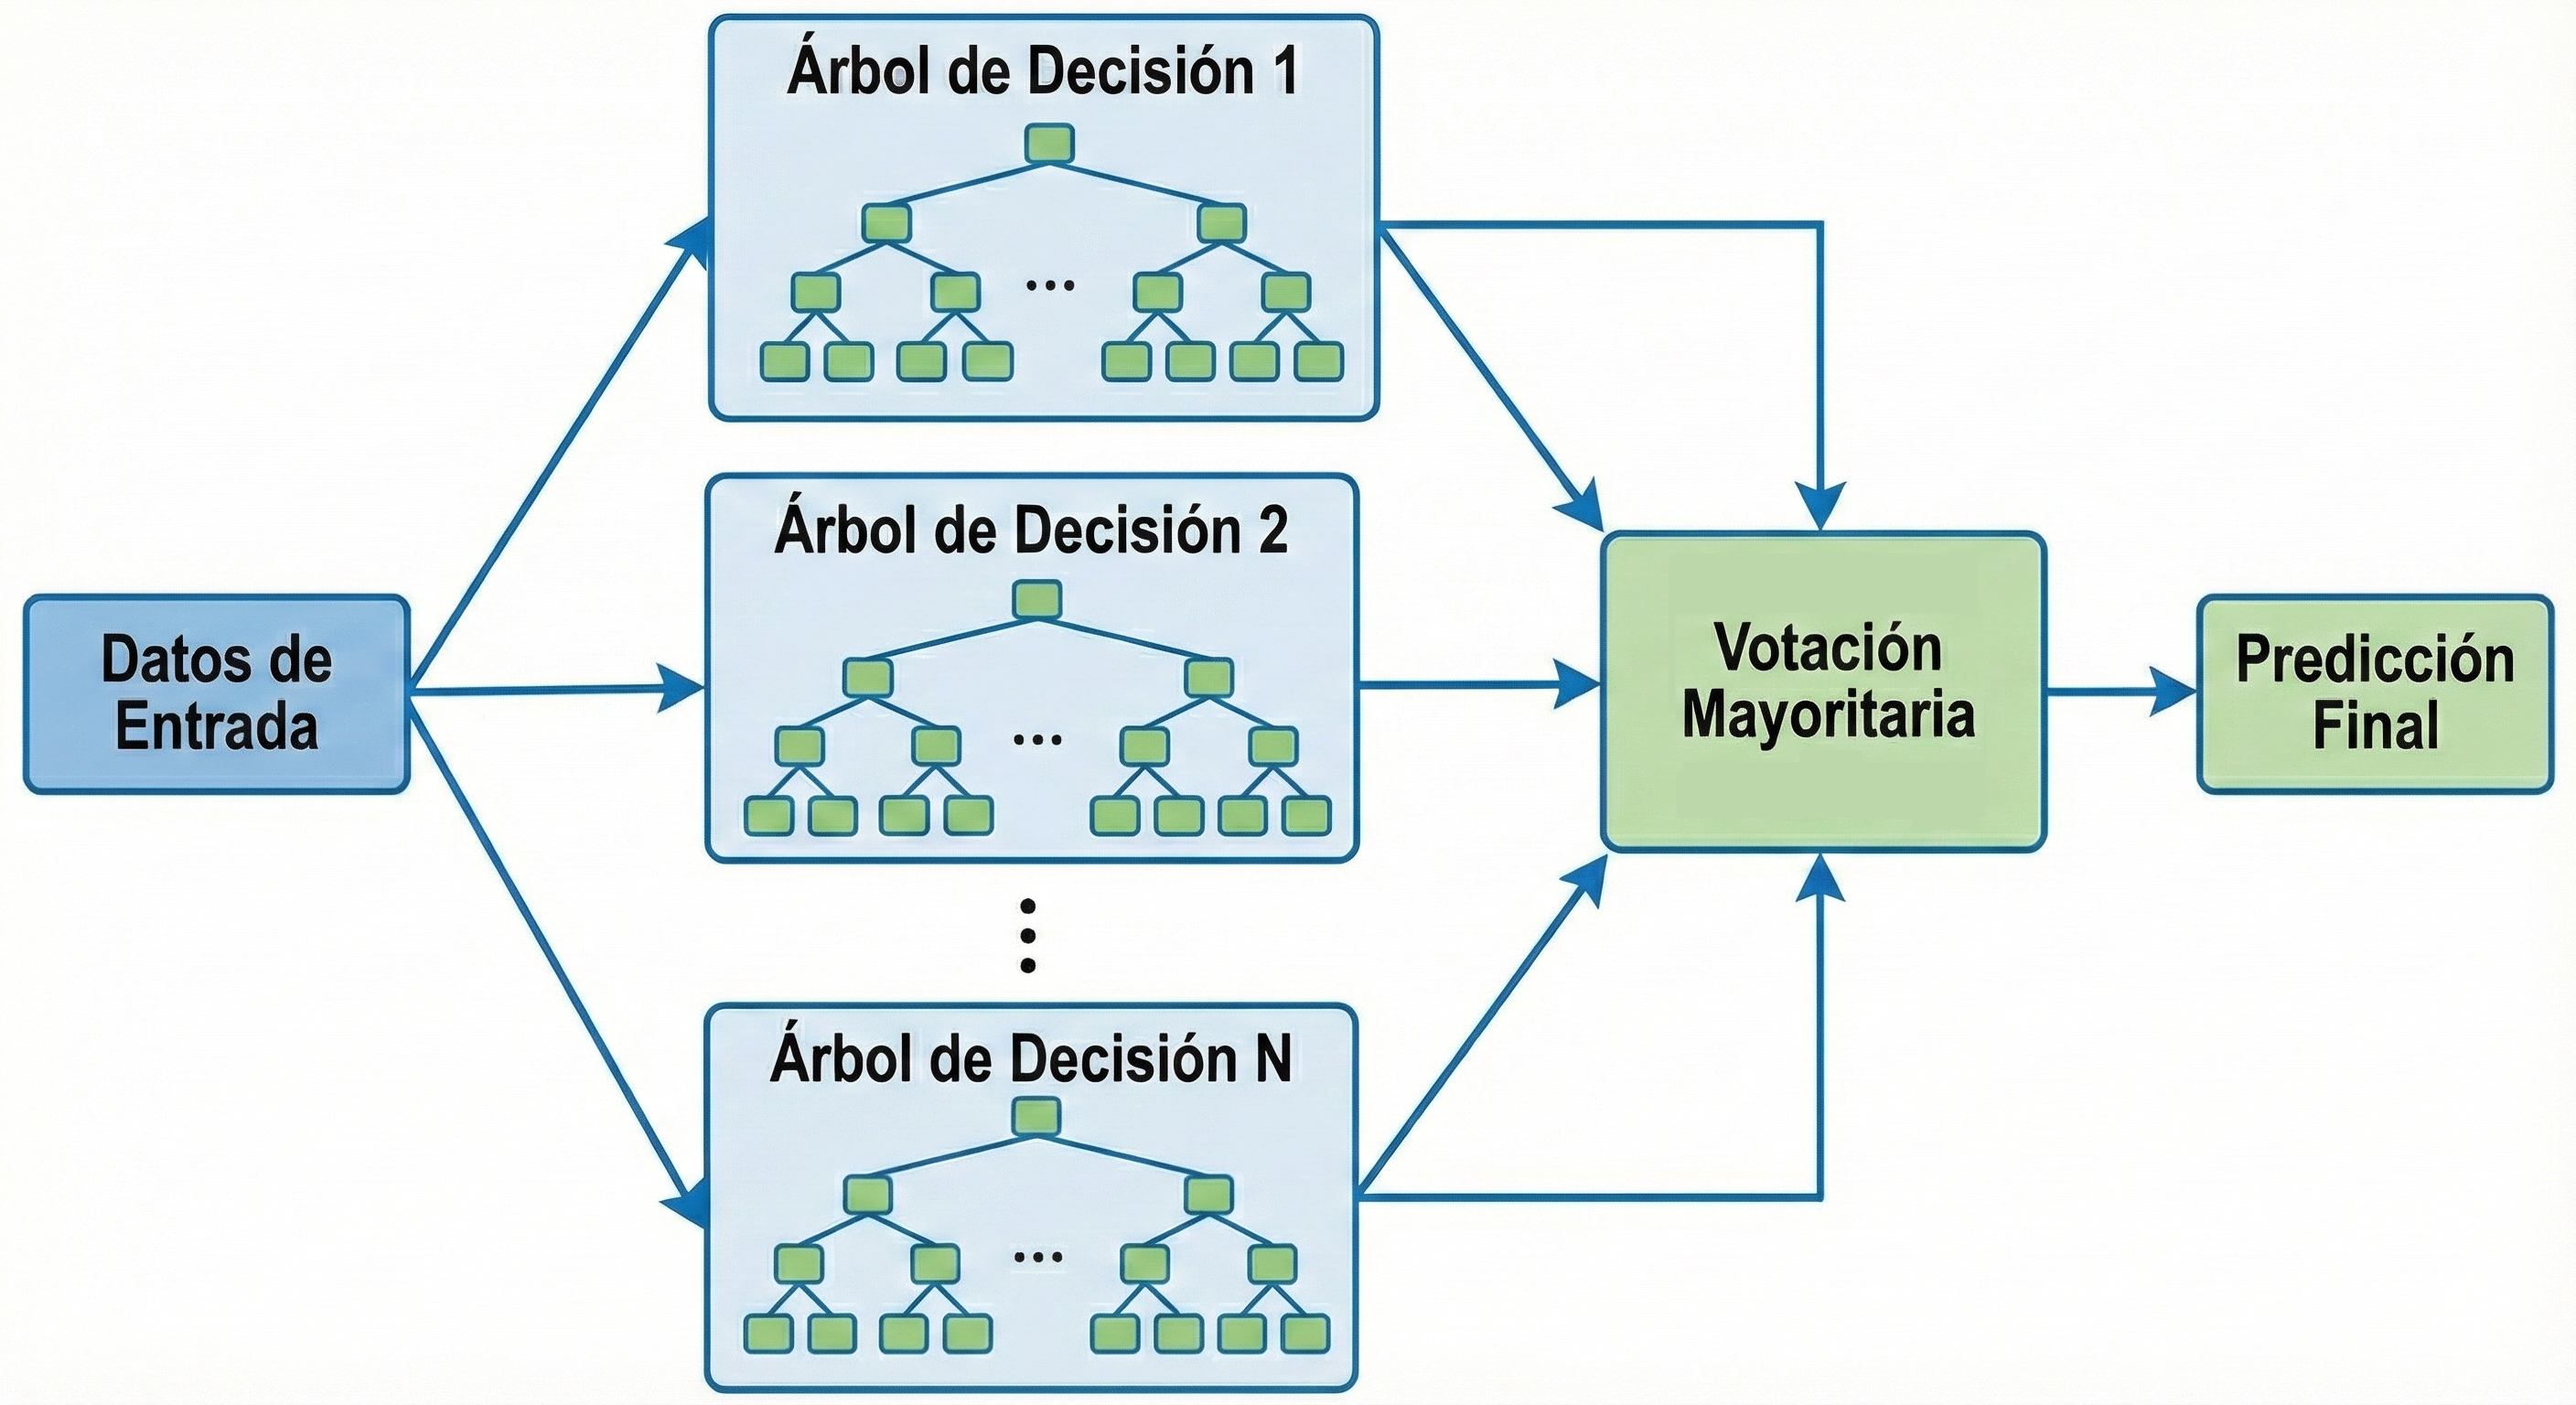
\includegraphics[width=0.9\textwidth]{Imagenes/rf_architecture.png}
	\caption{Arquitectura del clasificador Random Forest. El diagrama ilustra el mecanismo de ensamble: múltiples árboles de decisión ($Tree_1 \dots Tree_n$) procesan la entrada independientemente. La clase final se determina mediante la mayoría de votos (Majority Voting), lo que reduce la varianza y mejora la generalización del modelo.}
	\label{fig:rf_architecture}
\end{figure}

Como se ilustra en la Figura \ref{fig:rf_architecture}, esta estrategia de doble aleatorización reduce significativamente la correlación entre los árboles individuales y mitiga eficazmente el riesgo de sobreajuste (\textit{overfitting}), resultando en un modelo con una alta capacidad de generalización. Adicionalmente, Random Forest proporciona estimaciones automáticas de la importancia de cada característica, lo cual es valioso para interpretar qué aspectos de los movimientos oculares son más discriminativos para la identificación de individuos.
	% --- CAPÍTULO III ---
\chapter{Marco Metodológico}

Este capítulo describe el marco metodológico de la investigación: el diseño experimental, el sistema de captura implementado y las técnicas de procesamiento de señales utilizadas.

\section{Diseño y Tipo de Investigación}

\subsection{Enfoque Cuantitativo}

La presente investigación adopta un enfoque cuantitativo, sustentado en la recolección sistemática de datos numéricos y su posterior análisis mediante técnicas estadísticas y computacionales.
Esta elección metodológica se justifica por la naturaleza física y medible de las variables bajo estudio: posiciones espaciales del ojo expresadas en coordenadas $(x, y)$, velocidades angulares (en °/s), aceleraciones, y otras métricas cinemáticas que describen la dinámica del sistema oculomotor.
El uso de variables numéricas permite cuantificar de manera precisa los fenómenos físicos involucrados en el movimiento ocular.
Según Ramírez et al. \cite{ramirez2004}, el enfoque cuantitativo es apropiado cuando se busca establecer patrones de comportamiento, probar hipótesis y generalizar resultados a partir de muestras representativas mediante el análisis estadístico.
Las trayectorias oculares registradas se traducen en series temporales multidimensionales que pueden ser analizadas mediante herramientas matemáticas rigurosas.
Las características extraídas —tales como la velocidad pico de los sacádicos, el índice de suavidad (Jerk), la dimensión fractal de Higuchi, y las variaciones del diámetro pupilar— constituyen descriptores cuantitativos que permiten:

\begin{itemize}
	\item Caracterizar objetivamente el comportamiento oculomotor de cada participante
	\item Comparar estadísticamente las diferencias individuales
	\item Aplicar algoritmos de aprendizaje automático para la clasificación de patrones
	\item Validar la consistencia de las mediciones mediante análisis de precisión y reproducibilidad
\end{itemize}

Este enfoque sigue los principios de la física experimental, donde los fenómenos naturales se describen mediante modelos matemáticos y se validan a través de la replicabilidad y el análisis cuantitativo de los resultados obtenidos.

\subsection{Diseño Experimental}

El estudio se enmarca dentro de un diseño experimental de tipo controlado, en el cual se manipulan deliberadamente las variables independientes para observar su efecto sobre las variables dependientes del sistema oculomotor.
Específicamente, se diseñaron estímulos visuales estandarizados que permiten registrar y analizar las respuestas oculares bajo condiciones replicables.

\subsubsection{Variables del estudio}

El diseño experimental se estructura en torno a las siguientes variables:

\textbf{Variables independientes (manipuladas):}
\begin{itemize}
	\item \textit{Posición espacial del estímulo visual}: Una cuadrícula de $3 \times 3$ puntos que cubren el campo visual de la pantalla, generando 9 posiciones discretas que provocan movimientos sacádicos dirigidos.
	\item \textit{Duración de presentación del estímulo}: Cada punto permanece visible durante 2 segundos, tiempo suficiente para garantizar la estabilización de la fijación ocular según los criterios establecidos por Duchowski \cite{duchowski2017}.
	\item \textit{Secuencia de presentación}: Los estímulos se presentan siguiendo un orden determinado (de izquierda a derecha, de arriba hacia abajo), lo que induce un patrón predecible de movimientos oculares.
\end{itemize}

\textbf{Variables dependientes (observadas):}
\begin{itemize}
	\item Coordenadas espaciales del centroide de la pupila $(x_p(t), y_p(t))$ en función del tiempo
	\item Velocidad angular del movimiento ocular $v(t)$ [°/s]
	\item Aceleración angular $a(t)$ [°/s$^2$]
	\item Índice de suavidad del movimiento (Jerk) $J(t)$ [°/s$^3$]
	\item Diámetro pupilar $d(t)$ [mm] y su tasa de cambio
	\item Duración de las fijaciones y características de los movimientos sacádicos
\end{itemize}

\textbf{Variables controladas:}
\begin{itemize}
	\item Distancia sujeto-pantalla: $60 \pm 1$ cm
	\item Resolución y frecuencia de muestreo de la cámara
	\item Características físicas del estímulo (tamaño, contraste, color de fondo)
\end{itemize}

Este diseño permite establecer relaciones causales entre los estímulos presentados y las respuestas oculomotoras registradas, asegurando la validez interna del experimento mediante el control riguroso de factores que podrían introducir variabilidad no deseada en las mediciones.

\section{Sistema Experimental y Herramientas}

\subsection{Hardware e Instrumentación}

El sistema experimental desarrollado integra componentes de hardware que permiten la captura, procesamiento y almacenamiento de datos oculométricos en tiempo real.

\subsubsection{Equipo de cómputo}

El procesamiento de las señales oculares requiere capacidad computacional suficiente para ejecutar algoritmos de visión por computadora y aprendizaje automático en tiempo real.
El equipo utilizado presenta las siguientes características:

\begin{itemize}
	\item \textbf{Procesador}: Intel Core i7 de 11ª generación (8 núcleos, 16 hilos)
	\item \textbf{Memoria RAM}: 20 GB DDR4 a 3200 MHz
	\item \textbf{Sistema operativo}: Ubuntu 24.04 LTS (distribución Linux optimizada para desarrollo científico)
	\item \textbf{Almacenamiento}: SSD de 512 GB para lectura/escritura rápida de datos
	\item \textbf{Tarjeta gráfica}: GPU integrada Intel (utilizada para acelerar operaciones de procesamiento de imágenes)
\end{itemize}

Este equipo proporciona el poder de cómputo necesario para:
\begin{enumerate}
	\item Procesar flujos de video a 30-120 FPS en tiempo real
	\item Ejecutar algoritmos de detección y extracción de características
	\item Entrenar y validar modelos de aprendizaje automático
	\item Almacenar y gestionar grandes volúmenes de datos experimentales
\end{enumerate}

\begin{figure}[H]
	\centering
	\includegraphics[width=0.7\textwidth]{Imagenes/pc.jpg}
	\caption{Estación de trabajo utilizada para el procesamiento de datos y entrenamiento de la red neuronal.
		El equipo operó bajo entorno Linux (Ubuntu 24.04 LTS) para maximizar la eficiencia en la gestión de procesos en tiempo real.}
	\label{fig:computador_specs}
\end{figure}

\subsubsection{Sistema de captura de video}

La captura de imágenes del ojo se realizó mediante un módulo de cámara infrarroja especializado para visión artificial, basado en el sensor GC0308, cuyas especificaciones técnicas se detallan a continuación:

\begin{itemize}
	\item \textbf{Sensor}: GalaxyCore GC0308 (CMOS de 1/6.5 pulgadas)
	\item \textbf{Espectro de operación}: Infrarrojo cercano (NIR) con sensibilidad pico a 850 nm (sin filtro IR-cut)
	\item \textbf{Resolución operativa}: 320 $\times$ 240 píxeles (QVGA) para maximizar la tasa de cuadros
	\item \textbf{Frecuencia de muestreo}: Configurada a 120 FPS constantes
	\item \textbf{Interfaz de datos}: USB 2.0 de alta velocidad
	\item \textbf{Formato de salida}: MJPEG
	\item \textbf{Enfoque}: Lente de enfoque fijo manual (montura M12) ajustado para macro-distancia
\end{itemize}

\begin{figure}[H]
	\centering
	\includegraphics[width=0.6\textwidth]{Imagenes/gc0308.png} 
	\caption{Módulo de cámara con sensor GalaxyCore GC0308 adaptado para visión infrarroja cercana (NIR).
		Se observa la lente con montura M12 ajustable.}
	\label{fig:camara_gc0308}
\end{figure}

Se seleccionó una frecuencia de muestreo operativa de 120 Hz fundamentada en el teorema de muestreo de Nyquist-Shannon.
Dado que el ancho de banda fisiológico de los movimientos oculares sacádicos convencionales se sitúa en el rango de 20-25 Hz, una tasa de 120 FPS no solo satisface la condición de Nyquist ($120 > 50$), sino que proporciona un factor de sobremuestreo significativo.
Esto permite una reconstrucción temporal fidedigna de la dinámica ocular, minimizando el desenfoque de movimiento (\textit{motion blur}) durante las aceleraciones rápidas del ojo.

\textbf{Configuración geométrica y validez de la captura:}

A diferencia de los sistemas remotos, el dispositivo se configuró como un sistema montado en cabeza.
La cámara se acopló mecánicamente a la estructura de unos lentes, ubicada específicamente en la parte inferior derecha del campo visual y orientada con un ángulo de elevación hacia el globo ocular derecho.
Esta configuración de proximidad (distancia focal $< 5$ cm) garantiza que la región de interés (ROI) ocupe la totalidad del sensor.
A pesar de utilizar una resolución QVGA ($320 \times 240$), la densidad de píxeles efectiva sobre el área de la pupila es superior a la de una cámara HD ubicada a distancia.
La imagen resultante contiene exclusivamente información del ojo, eliminando ruido del entorno y reduciendo la carga computacional en el post-procesamiento, lo que facilita la detección precisa del centroide pupilar.

\subsection{Entorno y Condiciones de Iluminación}

El control de las condiciones ambientales es fundamental para garantizar la reproducibilidad de las mediciones y la calidad de las imágenes capturadas, particularmente cuando se utiliza el método de pupila oscura descrito en el marco teórico (Capítulo 2).

\subsubsection{Configuración espacial}

La configuración geométrica del sistema se estandarizó para todos los participantes:

\begin{itemize}
	\item \textbf{Distancia sujeto-pantalla}: 60 cm (medida desde la posición promedio de los ojos hasta el centro de la pantalla)
	\item \textbf{Altura de la pantalla}: Ajustada de manera que el centro de la pantalla coincida con la altura de los ojos del participante en posición erguida
	\item \textbf{Ángulo de visión}: 0° (pantalla perpendicular a la línea de visión primaria)
	\item \textbf{Posición de la cámara}: Montada en la parte inferior derecha de los lentes, apuntando aproximadamente a 45° hacia el ojo
\end{itemize}

Esta distancia de 60 cm fue seleccionada considerando que:
\begin{enumerate}
	\item Es una distancia ergonómica estándar para el trabajo frente a pantallas según las normas ISO 9241-5
	\item Maximiza la resolución angular del sistema de seguimiento sin comprometer la comodidad del participante
\end{enumerate}

\subsubsection{Control de iluminación}

Para implementar eficazmente el método de pupila oscura y maximizar el contraste entre la pupila y el iris, se establecieron las siguientes condiciones de iluminación:

\begin{itemize}
	\item \textbf{Iluminación ambiental}: Nivel de iluminancia controlado entre 500-900 lux, correspondiente a condiciones de oficina estándar.
	Todos los datos se recopilaron en este rango de lux, se corroboró usando un luxómetro UNIT UT383.
\end{itemize}

\textbf{Método de pupila oscura:} Gracias a la sensibilidad espectral del sensor GC0308 en el rango del infrarrojo cercano (sin filtro IR-cut), este estudio implementa el método de pupila oscura aprovechando la iluminación ambiental como fuente pasiva.
A diferencia de los sensores que operan exclusivamente en el espectro visible, este dispositivo capta la radiación infrarroja del entorno, la cual es absorbida eficientemente por la retina pero reflejada por el iris y la esclera.
Este fenómeno físico maximiza el contraste natural de la imagen, haciendo que la pupila aparezca significativamente más oscura sin necesidad de emisores activos (LEDs), lo que optimiza la segmentación mediante las técnicas de umbralización detalladas en la sección~\ref{sec:segmentacion}.

\subsection{Herramientas de Software}

El pipeline de procesamiento, desde la adquisición de imágenes hasta la clasificación de patrones, se implementó íntegramente en Python 3.10, seleccionado por su amplio ecosistema de bibliotecas científicas y su capacidad para prototipado rápido de algoritmos.

\subsubsection{Procesamiento de imágenes y visión por computadora}

\begin{itemize}
	\item \textbf{OpenCV (cv2) 4.8.0}: Biblioteca fundamental para la captura de video en tiempo real, aplicación de filtros de preprocesamiento (Gaussian, Bilateral), operaciones morfológicas, detección de contornos, y transformaciones geométricas.
	Esta biblioteca implementa eficientemente los algoritmos descritos en el marco teórico para la segmentación de la pupila.
	\item \textbf{Ultralytics YOLOv8 8.0.x}: Framework de aprendizaje profundo utilizado para la implementación, entrenamiento y validación de la red neuronal convolucional encargada de la detección y seguimiento de la pupila.
	Su integración permitió inferencias de alta velocidad (tiempo real) con el modelo personalizado.
	\item \textbf{NumPy 1.24.3}: Biblioteca fundamental para operaciones numéricas eficientes sobre matrices multidimensionales.
	Se utilizó extensivamente para:
	\begin{itemize}
		\item Manipulación de arrays de imágenes (tensores de dimensión $H \times W \times C$)
		\item Cálculo de derivadas numéricas para obtener velocidad, aceleración y Jerk
		\item Operaciones de álgebra lineal (productos matriciales, descomposiciones)
	\end{itemize}
\end{itemize}

\subsubsection{Procesamiento de señales}

\begin{itemize}
	\item \textbf{SciPy 1.11.2}: Conjunto de herramientas para computación científica que se empleó para:
	\begin{itemize}
		\item Implementación del filtro Savitzky-Golay (\texttt{scipy.signal.savgol\_filter})
		\item Cálculo de transformadas de Fourier para análisis frecuencial
		\item Interpolación de datos mediante splines cúbicos
		\item Optimización de parámetros mediante métodos de mínimos cuadrados
	\end{itemize}
\end{itemize}

\subsubsection{Análisis estadístico y visualización}

\begin{itemize}
	\item \textbf{Pandas 2.0.3}: Biblioteca para manipulación y análisis de datos estructurados.
	Se utilizó para:
	\begin{itemize}
		\item Organización de las características extraídas en DataFrames
		\item Cálculo de estadísticas descriptivas (media, desviación estándar, cuartiles)
		\item Exportación de resultados a formatos CSV y Excel
	\end{itemize}
	
	\item \textbf{Matplotlib 3.7.2} y \textbf{Seaborn 0.12.2}: Bibliotecas complementarias para visualización de datos.
	Se emplearon para:
	\begin{itemize}
		\item Generación de gráficos de trayectorias oculares
		\item Visualización de distribuciones de características mediante histogramas y boxplots
		\item Creación de matrices de confusión para evaluar los clasificadores
		\item Gráficos de la secuencia principal (velocidad vs. amplitud de sacádicos)
	\end{itemize}
\end{itemize}

\subsubsection{Aprendizaje automático}

\begin{itemize}
	\item \textbf{Scikit-learn 1.3.0}: Biblioteca integral de aprendizaje automático que proporciona implementaciones eficientes de los algoritmos descritos en el marco teórico:
	\begin{itemize}
		\item \texttt{LinearDiscriminantAnalysis}: Para reducción de dimensionalidad preservando la separabilidad entre clases
		\item \texttt{SVC}: Máquinas de Vectores de Soporte con kernel RBF para clasificación no lineal
		\item \texttt{RandomForestClassifier}: Clasificador basado en ensambles de árboles de decisión
		\item \texttt{StandardScaler}: Normalización de características para evitar sesgos por diferencias de escala
		\item \texttt{train\_test\_split}: División estratificada de datos en conjuntos de entrenamiento y prueba
		\item Métricas de evaluación: \texttt{accuracy\_score}, \texttt{classification\_report}, \texttt{confusion\_matrix}
	\end{itemize}
\end{itemize}


\subsection{Disponibilidad del Código}
El código fuente completo del sistema desarrollado, incluyendo los scripts de procesamiento, análisis y visualización, está disponible públicamente en el repositorio de GitHub: \url{https://github.com/LilkongW/Tesis3D.git}. 

Este repositorio contiene:
\begin{itemize}
	\item Los scripts de captura y procesamiento de imágenes
	\item El modelo YOLOv8 entrenado para detección pupilar
	\item Los algoritmos de extracción de métricas biométricas
	\item Los scripts de análisis estadístico y generación de gráficos
\end{itemize}

\subsection{Arquitectura del Flujo de Datos (Pipeline)}

El sistema se diseñó bajo una arquitectura modular secuencial compuesta por tres etapas de procesamiento, cada una gestionada por scripts específicos desarrollados en Python.
Este flujo garantiza la trazabilidad de los datos desde la captura cruda hasta el análisis estadístico final.
La Figura \ref{fig:pipeline_flujo} ilustra la secuencia de transformación de los datos, vinculando los algoritmos descritos con los módulos de software implementados.

\begin{figure}[H]
	\centering
	\includegraphics[width=\textwidth, height=20cm, keepaspectratio]{Imagenes/flow.png}
	\caption{Diagrama de flujo de la arquitectura de procesamiento de datos.
		Se ilustra la secuencia desde la captura de video hasta la generación de resultados biométricos.}
	\label{fig:pipeline_flujo}
\end{figure}

Adicionalmente, la Tabla \ref{tab:flujo_datos} detalla la función específica de cada módulo de software dentro del repositorio del proyecto, especificando las entradas y salidas de cada etapa.

\begin{table}[H]
	\centering
	\caption{Descripción funcional de los módulos de software del sistema.}
	\vspace{0.2cm}
	\resizebox{\textwidth}{!}{%
		\begin{tabular}{lp{5cm}p{3.5cm}p{3.5cm}}
			\toprule
			\textbf{Etapa} & \textbf{Módulo (Script)} & \textbf{Entrada (Input)} & \textbf{Salida (Output)} \\
			\midrule
			\textbf{1. Extracción} & \texttt{main.py} \newline \texttt{eye\_tracker\_utils.py} & Videos del ojo ($120$ FPS) & Archivos \texttt{\_data.csv} con centroides y vector mirada $(g_x, g_y, g_z)$. \\
			\midrule
			\textbf{2. Métricas} & \texttt{Generar\_Metricas.py} & Series temporales de posición ($P(t)$) & Dataset \texttt{BIOMETRIC.csv} con 18 descriptores (Jerk, HFD, etc.) \\
			\midrule
			\textbf{3. Análisis} & \texttt{Analizar\_Metricas.py} & Dataset Biométrico consolidado & Gráficos de Radar, Clusters LDA y Matrices de Confusión. \\
			\bottomrule
		\end{tabular}
	}
	\label{tab:flujo_datos}
\end{table}

\section{Protocolo de Adquisición de Datos}

\subsection{Población y Muestra}

\subsubsection{Caracterización de la población objetivo}

La población objetivo de este estudio la conforman adultos jóvenes sin patologías oculomotoras diagnosticadas, residentes en Mérida (Venezuela).
Este grupo demográfico fue seleccionado por presentar características oculomotoras estables y bien documentadas en la literatura científica, lo que facilita la comparación de los resultados obtenidos con estudios previos.

\subsubsection{Criterios de selección}

Para garantizar la homogeneidad de la muestra y la validez de las mediciones, se establecieron los siguientes criterios de inclusión y exclusión:

\textbf{Criterios de inclusión:}
\begin{itemize}
	\item Edad comprendida entre 20 y 35 años
	\item Ausencia de patologías oculares diagnosticadas (cataratas, glaucoma, desprendimiento de retina)
	\item Comprensión de las instrucciones del experimento
\end{itemize}

\subsubsection{Tamaño y composición de la muestra}

La muestra final consistió en 15 participantes (N = 15), seleccionados mediante muestreo no probabilístico por conveniencia.
La composición demográfica fue:

\begin{itemize}
	\item \textbf{Edad}: Media de 25.3 años, desviación estándar de 3.7 años
	\item \textbf{Sexo}: 11 hombres (73.3\%) y 4 mujeres (26.7\%)
	\item \textbf{Corrección visual}: 8 participantes con visión normal (53.3\%) y 7 con corrección óptica (lentes o lentes de contacto, 46.7\%)
\end{itemize}

Este tamaño de muestra, aunque limitado, es consistente con estudios piloto en el campo de la biometría oculomotora.
Investigaciones previas como las de Komogortsev et al. \cite{komogortsev2010} han demostrado que muestras de 10-20 participantes son suficientes para validar la viabilidad de sistemas de seguimiento ocular y establecer la singularidad de patrones oculomotores individuales en condiciones controladas.
A continuación, la Tabla \ref{tab:participantes_detalle} detalla las condiciones específicas registradas para cada uno de los 15 participantes durante las sesiones experimentales.

\begin{table}[H]
	\centering
	\caption{Caracterización demográfica y condiciones ambientales por participante con incertidumbres asociadas.}
	\vspace{0.2cm}
	\begin{tabular}{ccccc}
		\toprule
		\textbf{Sujeto} & \textbf{Edad (años)} & \textbf{Distancia (cm)} & \textbf{Iluminancia (Lux)} \\
		\midrule
		P01 & 24 & 59 & 585 \\
		P02 & 26  & 60 & 620 \\
		P03 & 22 & 60 & 550 \\
		P04 & 29  & 58 & 710 \\
		P05 & 25 & 60 & 680 \\
		P06 & 31  & 60 & 850 \\
		P07 & 23  & 59 & 595 \\
		P08 & 27  & 60 & 640 \\
		P09 & 21 & 59 & 520 \\
		P10 & 35 & 60 & 890 \\
		P11 & 28  & 60 & 730 \\
		P12 & 24 & 60 & 615 \\
		P13 & 30  & 59 & 800 \\
		P14 & 22  & 60 & 560 \\
		P15 & 26  & 60 & 675 \\
		\bottomrule
	\end{tabular}
	\label{tab:participantes_detalle}
	\vspace{0.2cm}
	\begin{minipage}{0.9\textwidth}
		\footnotesize
		\textbf{Consideraciones Metrológicas:}
		\begin{itemize}
			\item \textbf{Distancia ($\pm 1$ cm):} Medición realizada con cinta métrica comercial (resolución 1 mm).
			Se asigna una incertidumbre expandida de $\pm 1$ cm para compensar el error de posicionamiento de la cabeza (paralaje y micro-movimientos).
			\item \textbf{Iluminancia ($\pm \Delta$):} Medición realizada con luxómetro digital UNI-T UT383.
			Según especificaciones del fabricante, la precisión instrumental en el rango $<9999$ Lux es de $\pm(4\% \text{ lectura} + 8 \text{ dígitos})$.
		\end{itemize}
	\end{minipage}
\end{table}

\subsubsection{Consideraciones éticas}

Todos los participantes fueron informados sobre los objetivos del estudio, los procedimientos a seguir, y el uso que se daría a los datos recolectados.
Se garantizó la confidencialidad de la información personal mediante la asignación de códigos anónimos (P01-P15).
No se registraron imágenes que permitieran la identificación facial de los participantes, únicamente las regiones oculares necesarias para el análisis.

\subsection{Diseño del Estímulo Visual}

\subsubsection{Cuadrícula de calibración y prueba (Grid 3×3)}

El estímulo visual consistió en una cuadrícula regular de $3 \times 3$ puntos distribuidos uniformemente sobre el área activa del monitor.
La posición de los puntos se calculó dividiendo la resolución de pantalla ($W \times H$) en tres segmentos iguales tanto horizontal como verticalmente, situando cada estímulo en el centro geométrico de cada celda resultante.
Para una resolución estándar de $1920 \times 1080$ píxeles, esto resulta en una separación constante entre centros de 640 píxeles en el eje horizontal y 360 píxeles en el eje vertical.

\begin{figure}[htbp]
	\centering
	\caption{Esquema de la cuadrícula de estímulos visuales $3 \times 3$. Los números indican el orden secuencial de presentación.
		Para una resolución de $1920 \times 1080$, la separación horizontal entre estímulos ($\Delta x$) es de 640 px y la vertical ($\Delta y$) es de 360 px.}
	\label{fig:grid_stimulus}
\end{figure}

\textbf{Características geométricas y cromáticas del estímulo:}

\begin{itemize}
	\item \textbf{Número de puntos}: 9 (matriz de $3 \times 3$)
	\item \textbf{Forma y dimensión}: Círculos sólidos con un radio de 30 píxeles (diámetro total de 60 píxeles).
	A una distancia de observación aproximada de 60 cm, esto subtiende un ángulo visual de $\approx 1.5^\circ$, garantizando una estimulación foveal clara.
	\item \textbf{Cromaticidad del estímulo}: Rojo puro de máxima intensidad (Espacio de color BGR: 0, 0, 255; RGB: 255, 0, 0).
	\item \textbf{Fondo}: Negro absoluto (RGB: 0, 0, 0). Se seleccionó un fondo de mínima luminancia para maximizar el contraste con el estímulo y eliminar distracciones visuales periféricas, facilitando la segmentación de la pupila al reducir reflejos externos en la córnea.
	\item \textbf{Distribución espacial}: 
	\begin{itemize}
		\item Separación Horizontal: $W/3$ (640 px), induciendo sacádicos de amplitud media-grande ($\approx 15^\circ - 20^\circ$).
		\item Separación Vertical: $H/3$ (360 px), induciendo sacádicos verticales de amplitud controlada.
	\end{itemize}
\end{itemize}

Esta configuración espacial fuerza al sistema oculomotor a realizar movimientos sacádicos de amplitudes conocidas, cubriendo tanto el rango lineal como la región de saturación de la \textit{Main Sequence} (Ecuación 2.1), lo cual es fundamental para validar la dinámica del movimiento ocular capturado.

\subsubsection{Secuencia temporal de presentación}

Los estímulos se presentaron siguiendo una secuencia determinista controlada por software, garantizando la repetibilidad del experimento entre sujetos:

\begin{enumerate}
	\item \textbf{Patrón de barrido}: La activación siguió un orden de lectura occidental (izquierda a derecha, arriba hacia abajo):
	\begin{itemize}
		\item Fila superior ($y=H/6$): Posiciones 1, 2, 3
		\item Fila media ($y=H/2$): Posiciones 4, 5, 6
		\item Fila inferior ($y=5H/6$): Posiciones 7, 8, 9
	\end{itemize}
	
	Este patrón reduce la carga cognitiva del participante al hacer predecible la ubicación del siguiente objetivo, permitiendo enfocarse puramente en la tarea motora visual.
	\item \textbf{Temporización estricta}: Cada estímulo permaneció estático en pantalla durante un intervalo exacto de $T = 2000$ ms (2 segundos).
	Este intervalo se seleccionó considerando la fisiología del ojo:
	\begin{itemize}
		\item \textit{Latencia sacádica}: $\approx 200$ ms.
		\item \textit{Tiempo de vuelo}: $30-100$ ms.
		\item \textit{Fijación estable}: El tiempo restante ($>1.7$ s) asegura la captura de suficientes fotogramas estables para el cálculo preciso del centroide pupilar promedio en cada posición.
	\end{itemize}
	
	\item \textbf{Sincronización de eventos}: El cambio de posición del estímulo se programó para ser instantáneo (transición en el siguiente refresco de pantalla), generando un estímulo tipo escalón (step stimulus) ideal para medir la respuesta al impulso del sistema oculomotor.
\end{enumerate}

\begin{figure}[ht!]  
	\centering
	\includegraphics[width=0.7\textwidth]{Imagenes/experimento.png}
	\caption{Visualización del protocolo de estímulos (Experimento 1). La matriz de $3 \times 3$ puntos rojos sobre fondo negro se utiliza para inducir movimientos sacádicos controlados.
		Los puntos aparecen de forma secuencial con una duración de 2 segundos por posición, cubriendo la totalidad del campo de visión efectivo.}
	\label{fig:experimento_grid}
\end{figure}

\subsection{Procedimiento Experimental}

El protocolo experimental se diseñó para garantizar condiciones estandarizadas y replicables entre todos los participantes ($N=15$).
Cada sesión individual tuvo una duración aproximada de 10 minutos e incluyó las siguientes etapas secuenciales:

\subsubsection{Fase 1: Recepción y consentimiento informado}

\begin{enumerate}
	\item \textbf{Bienvenida}: Se recibió al participante y se le explicó verbalmente el propósito general del estudio: analizar la dinámica oculomotora mediante visión artificial.
	\item \textbf{Registro de metadatos}: Se completó una ficha técnica con las variables de control: Edad, Sexo y Tipo de corrección visual (gafas/lentes de contacto), dado que el 46.7\% de la muestra utilizaba algún tipo de ayuda óptica.
\end{enumerate}

\subsubsection{Fase 2: Colocación del dispositivo y configuración óptica}

Dado que el sistema de captura es del tipo \textit{head-mounted} (montado en la cabeza), el procedimiento de ajuste difiere de los sistemas remotos tradicionales:

\begin{enumerate}
	\item \textbf{Colocación del dispositivo}: El participante se colocó la montura de gafas que soporta la cámara GC0308.
	Se verificó que la estructura fuera cómoda y estable, asegurando que la cámara quedara ubicada en el cuadrante inferior derecho del campo visual, apuntando hacia el ojo en un ángulo de elevación (aprox. $30^\circ$).
	\item \textbf{Ajuste del ROI (Región de Interés)}: Mediante la visualización en tiempo real en el monitor de control, se ajustó mecánicamente el brazo flexible de la cámara para centrar el ojo en la imagen de $320 \times 240$ píxeles, garantizando que la pupila se mantuviera dentro del encuadre incluso durante movimientos extremos hacia las esquinas.
	\item \textbf{Posicionamiento frente al estímulo}: El participante se sentó frente al monitor.
	Se ajustó la altura de la silla para alinear los ojos con el centro de la pantalla y se fijó la distancia de observación a 60 cm (medida con cinta métrica) para asegurar que la geometría de los movimientos sacádicos correspondiera a los ángulos visuales calculados ($\approx 20^\circ$ horizontal).
\end{enumerate}

\subsubsection{Fase 3: Ejecución de la prueba principal}

El software de control (desarrollado en Python) gestionó la sincronización entre el estímulo y la captura:

\begin{enumerate}
	\item \textbf{Inicialización y Logs}: Al iniciar el script, se generó automáticamente un archivo CSV para registrar las marcas temporales (\textit{timestamps}) de cada cambio de estímulo.
	\item \textbf{Cuenta regresiva}: Se presentó una cuenta visual en pantalla (3-2-1) para preparar al sujeto.
	\item \textbf{Protocolo de adquisición}: Se ejecutó la matriz de 9 puntos.
	El sistema grabó video continuo a 120 FPS en formato MJPEG para evitar latencia, mientras registraba simultáneamente en el log la posición $(x,y)$ del punto rojo y el tiempo exacto de aparición.
	\item \textbf{Control de parpadeo}: Se instruyó a los participantes intentar no parpadear durante los 2 segundos de fijación activa, permitiéndolo libremente durante las transiciones si fuera necesario.
\end{enumerate}

\subsubsection{Fase 4: Repetición y consistencia de datos}

Para garantizar la robustez estadística y filtrar posibles artefactos (parpadeos involuntarios o pérdida de tracking), se realizó un diseño iterativo:

\begin{enumerate}
	\item Se realizaron 3 iteraciones (intentos) completas del experimento por cada participante.
	\item Entre iteraciones se estableció un intervalo de descanso aproximado de 10 segundos.
	\item El volumen total de datos adquiridos se calcula como:
	\[
	\text{Frames totales} = N_{\text{sujetos}} \times N_{\text{intentos}} \times (T_{\text{ensayo}} \times FPS)
	\]
	\[
	15 \times 3 \times (18\,\text{s} \times 120\,\text{fps}) \approx 97,200\,\text{imágenes oculares}
	\]
\end{enumerate}

Esta alta densidad temporal (120 Hz) proporciona suficiente información para reconstruir la curva de velocidad de los movimientos sacádicos con gran detalle.

\subsubsection{Fase 5: Cierre de la sesión}

\begin{enumerate}
	\item Se retiró el dispositivo del participante.
	\item Se verificó la integridad de los archivos de video (.avi/.mp4) y los logs de datos (.csv) antes de liberar al sujeto.
	\item Se agradeció la participación y se procedió a preparar el equipo de captura para el siguiente usuario.
\end{enumerate}

\section{Procesamiento Digital de Imágenes}
\label{sec:procesamiento_imagenes}

El procesamiento digital de imágenes constituye el núcleo del sistema de seguimiento ocular desarrollado.
Esta sección describe, desde una perspectiva algorítmica y matemática, cómo se transforman las imágenes RGB capturadas por la cámara en coordenadas precisas del centroide de la pupila.
El pipeline de procesamiento se divide en tres etapas fundamentales: preprocesamiento, segmentación y detección de la pupila, y mapeo de coordenadas.

\subsection{Preprocesamiento}

El objetivo del preprocesamiento es mejorar la calidad de las imágenes capturadas, reducir el ruido, y preparar los datos para los algoritmos de segmentación subsecuentes.
Las operaciones de preprocesamiento se aplican secuencialmente a cada fotograma capturado.

\subsubsection{Conversión a escala de grises}

Las imágenes RGB capturadas por la cámara son tensores tridimensionales de dimensión $H \times W \times 3$, donde $H = 720$ píxeles (altura), $W = 1280$ píxeles (ancho), y los tres canales corresponden a Rojo (R), Verde (G), y Azul (B).
Para simplificar el procesamiento posterior y reducir la carga computacional, las imágenes se convierten a escala de grises mediante la transformación:

\begin{equation}
	I_{\text{gray}}(x, y) = 0.2989 \cdot R(x, y) + 0.5870 \cdot G(x, y) + 0.1140 \cdot B(x, y)
\end{equation}

donde $I_{\text{gray}}(x, y)$ es la intensidad en escala de grises del píxel ubicado en la posición $(x, y)$, y los coeficientes reflejan la sensibilidad espectral del sistema visual humano (el canal verde contribuye más a la percepción de luminancia).
Esta transformación reduce el espacio de representación de 3 canales a 1 canal, pasando de $720 \times 1280 \times 3 = 2{,}764{,}800$ valores por fotograma a $720 \times 1280 = 921{,}600$ valores, lo cual acelera significativamente las operaciones subsecuentes sin pérdida de información relevante para la detección de la pupila.

\subsubsection{Reducción de ruido mediante filtrado}

Las imágenes capturadas por cámaras digitales inevitablemente contienen ruido, proveniente de fuentes como la sensibilidad del sensor, condiciones de baja iluminación, y artefactos de compresión.
Para suavizar estas fluctuaciones aleatorias de intensidad sin perder información estructural importante (como los bordes de la pupila), se aplicaron dos tipos de filtros complementarios:

\paragraph{Filtro Gaussiano}

El filtro Gaussiano es un filtro lineal de paso bajo que atenúa las componentes de alta frecuencia espacial (ruido) mediante una convolución con un kernel gaussiano bidimensional descrito por Giménez et al. \cite{gimenez2016aplicacion}:

\begin{equation}
	G(x, y) = \frac{1}{2\pi\sigma^2} \exp\left(-\frac{x^2 + y^2}{2\sigma^2}\right)
\end{equation}

donde $\sigma$ es la desviación estándar de la distribución gaussiana, que controla el grado de suavizado.
En este estudio se utilizó $\sigma = 1.5$ y un kernel de tamaño $5 \times 5$ píxeles.
La imagen filtrada se obtiene mediante:

\begin{equation}
	I_{\text{filtrada}}(x, y) = (I_{\text{gray}} * G)(x, y) = \sum_{i=-2}^{2} \sum_{j=-2}^{2} I_{\text{gray}}(x-i, y-j) \cdot G(i, j)
\end{equation}

\subsection{Segmentación y Detección de Pupila}
\label{sec:segmentacion}

El proceso de segmentación se implementó mediante un flujo de trabajo (pipeline) de visión artificial diseñado para operar con alta eficiencia temporal (120 FPS).
A diferencia de los métodos clásicos basados puramente en procesamiento de imagen, este estudio integra un modelo de aprendizaje profundo para la localización robusta, seguido de algoritmos geométricos para la precisión sub-pixel.

\subsubsection{Localización y Seguimiento de la Pupila mediante Deep Learning}

Para la localización robusta de la pupila frame a frame, se implementó una red neuronal convolucional basada en la arquitectura YOLOv8 (\textit{You Only Look Once}, versión 8).
A diferencia de los enfoques genéricos de detección de rostros, se optó por entrenar un modelo específico para la detección de la pupila en entornos infrarrojos cercanos (NIR).

\paragraph{Arquitectura y Entrenamiento (Fine-Tuning)}
Se seleccionó la variante YOLOv8n-seg (Nano), la arquitectura más ligera de la familia YOLO (3.2 millones de parámetros), para garantizar una inferencia en tiempo real compatible con la tasa de captura de 120 FPS.
El modelo no se utilizó de caja (\textit{out-of-the-box}), sino que se sometió a un proceso de transferencia de aprendizaje (\textit{fine-tuning}):

\begin{enumerate}
	\item \textbf{Conjunto de datos (Dataset)}: Se construyó un dataset personalizado utilizando fotogramas extraídos de los propios participantes del estudio durante la fase de calibración.
	Se etiquetaron manualmente 864 imágenes representativas que incluían variaciones en la apertura palpebral, reflejos corneales y distintas iluminaciones.
	\item \textbf{Configuración del entrenamiento}: El modelo pre-entrenado en el dataset COCO se re-entrenó durante 80 épocas con un tamaño de lote (batch size) de 16 y un optimizador SGD (Descenso de Gradiente Estocástico) con momentum de 0.937.
	\item \textbf{Validación}: El modelo resultante (\texttt{best.pt}) alcanzó una precisión media (mAP@50) superior al 98\% en el conjunto de validación, demostrando una capacidad de generalización robusta frente a la variabilidad inter-sujeto.
\end{enumerate}

Esta estrategia de entrenamiento específico resultó fundamental para mitigar la pérdida de seguimiento durante parpadeos o movimientos sacádicos rápidos, superando las limitaciones de los métodos tradicionales de visión artificial.

\paragraph{Inferencia en tiempo de ejecución}
Durante la fase experimental, el algoritmo opera de la siguiente manera para cada fotograma $I_t$:
\begin{enumerate}
	\item \textbf{Pre-recorte}: Se ajusta la relación de aspecto de la imagen de entrada a $320 \times 240$ para mantener la consistencia espacial con los datos de entrenamiento.
	\item \textbf{Inferencia}: El modelo predice un cuadro delimitador (bounding box) $B = (x_1, y_1, x_2, y_2)$ centrado en la pupila.
	\item \textbf{Filtrado y Expansión}: Se aceptan únicamente detecciones con una confianza $C \geq 0.7$.
	Las coordenadas predichas se expanden en 5 píxeles por lado (\textit{padding}) para definir la Región de Interés (ROI) final, asegurando que los bordes de la pupila se preserven íntegramente para la etapa de segmentación sub-pixel.
\end{enumerate}

\subsubsection{Pre-procesamiento y mejora de contraste}

Dado que la iluminación infrarroja puede generar histogramas de intensidad concentrados en rangos oscuros, se aplicaron técnicas de mejora de imagen antes de la segmentación.
Según se observa en la función \texttt{process\_frame} del algoritmo implementado:

\begin{enumerate}
	\item \textbf{Suavizado Gaussiano}: Se aplicó un filtro Gaussiano con kernel $(7 \times 7)$ para reducir el ruido de alta frecuencia del sensor CMOS.
	\item \textbf{Ecualización de Histograma Adaptativa (CLAHE)}: Se utilizó \textit{Contrast Limited Adaptive Histogram Equalization} con un límite de recorte (\textit{clip limit}) de 1.0 y una rejilla de $8 \times 8$.
	Esto maximiza el contraste local entre la pupila y el iris sin amplificar el ruido en las zonas homogéneas, lo cual es crítico para el método de pupila oscura.
\end{enumerate}

\subsubsection{Segmentación y Ajuste Geométrico}

En lugar de depender de operaciones morfológicas tradicionales que pueden deformar la forma de la pupila, se implementó un enfoque basado en la geometría de contornos:

\paragraph{1. Binarización}
Se aplicó una umbralización binaria invertida fija sobre la imagen mejorada por CLAHE:
\begin{equation}
	I_{\text{bin}}(x, y) = \begin{cases}
		255 & \text{si}\quad I_{\text{CLAHE}}(x, y) < T_{\text{fijo}} \\
		0 & \text{en caso contrario}
	\end{cases}
\end{equation}
Donde $T_{\text{fijo}}$ es un parámetro empírico (configurado en 14-20 niveles de intensidad) que separa la región negra profunda de la pupila del resto del ojo.

\paragraph{2. Optimización de Contornos por Ángulo}
Tras detectar los contornos, se seleccionó el contorno de mayor área.
Para eliminar irregularidades causadas por pestañas o reflejos (glints), se implementó un algoritmo de filtrado geométrico (\texttt{optimize\_contours\_by\_angle}).
Este algoritmo evalúa la suavidad de la curvatura calculando el coseno del ángulo entre vectores formados por puntos adyacentes del contorno:
\begin{equation}
	\cos \theta = \frac{\vec{v}_1 \cdot \vec{v}_2}{\|\vec{v}_1\| \|\vec{v}_2\|}
\end{equation}
Los puntos que generan cambios angulares abruptos (vértices agudos no compatibles con la curvatura de la pupila) son descartados como ruido.

\begin{algorithm}[H]
	\caption{Optimización de Contornos por Suavidad Angular}
	\label{alg:optimize_contours}
	\begin{algorithmic}[1]
		\Require Contorno original $C = \{P_1, P_2, \dots, P_N\}$, Umbral de suavidad $\tau$
		\Ensure Contorno optimizado $C_{opt}$
		\State $C_{opt} \gets \emptyset$
		\For{$i \gets 1$ \textbf{to} $N$}
		\State Obtener puntos adyacentes:
		\State $P_{prev} \gets C[(i-1) \pmod N]$
		\State $P_{curr} \gets C[i]$
		\State $P_{next} \gets C[(i+1) \pmod N]$
		
		\State Calcular vectores direccionales:
		\State $\vec{v}_1 \gets P_{curr} - P_{prev}$
		\State $\vec{v}_2 \gets P_{next} - P_{curr}$
		
		\State Calcular similitud angular (Coseno):
		\State $\cos \theta \gets \frac{\vec{v}_1 \cdot \vec{v}_2}{\|\vec{v}_1\| \|\vec{v}_2\|}$
		
		\State Filtrado geométrico:
		\If{$\cos \theta > \tau$} \Comment{El ángulo es suave (compatible con curvatura)}
		\State Agregar $P_{curr}$ a $C_{opt}$
		\Else
		\State Descartar $P_{curr}$ \Comment{Vértice agudo (ruido/pestaña)}
		\EndIf
		\EndFor
		\State \Return $C_{opt}$
	\end{algorithmic}
\end{algorithm}

\paragraph{3. Ajuste de Elipse (Least Squares Fitting)}
Finalmente, se ajustó una elipse a los puntos del contorno optimizado utilizando el método de mínimos cuadrados directos (\textit{Direct Least Squares fitting of Ellipses}).
Esto retorna el centroide con precisión sub-pixel $(x_c, y_c)$, los ejes mayor y menor, y el ángulo de rotación, proporcionando una estimación robusta de la posición de la pupila incluso ante oclusiones parciales.

\begin{figure}[htbp]
	\centering
	\includegraphics[width=1.0\textwidth]{Imagenes/preprocesamiento.png}
	\caption{Pipeline de procesamiento de imagen implementado. La secuencia muestra: (Arriba) Mejora de la imagen mediante escala de grises y realce de contraste CLAHE.
		(Abajo) Detección de la ROI con YOLOv8, binarización inversa adaptativa y superposición final del contorno elíptico ajustado sobre la imagen original.}
	\label{fig:pipeline_procesamiento}
\end{figure}

\subsection{Estimación del Vector de Mirada (Gaze Vector)}

A diferencia de los mapeos polinomiales 2D simples, este estudio implementó un modelo geométrico 3D simplificado para estimar la dirección de la mirada.
El algoritmo calcula un Centro del Modelo (aproximación del centro de rotación ocular o centro óptico virtual) mediante la intersección promedio de los vectores normales a la superficie del ojo a lo largo del tiempo.
Posteriormente, tal como se ilustra en la Figura~\ref{fig:vector_mirada}, el vector de mirada unitario $\hat{g}$ se calcula normalizando la diferencia entre el centro de la pupila detectado $\mathbf{p} = (x_p, y_p, 0)$ y el centro del modelo $\mathbf{c} = (x_c, y_c, z_c)$:

\begin{equation}
	\vec{v} = \mathbf{p} - \mathbf{c}, \quad \hat{g} = \frac{\vec{v}}{\|\vec{v}\|} = (g_x, g_y, g_z)
\end{equation}

Este enfoque vectorial permite calcular la cinemática angular de manera más fiel a la fisiología del ojo.

\begin{figure}[htbp]
	\centering
	\includegraphics[width=0.9\textwidth]{Imagenes/calculo_vector_mirada.png}
	\caption{Esquema de la estimación del vector de mirada. (Izquierda) Identificación del contorno pupilar.
		(Centro) Cálculo del centro del modelo ocular (punto azul) respecto al centroide de la pupila.
		(Derecha) Proyección del vector de mirada resultante (línea roja) en el espacio 3D.}
	\label{fig:vector_mirada}
\end{figure}

\subsubsection{Validación y Justificación del Enfoque Híbrido}

La selección de una arquitectura basada en aprendizaje profundo (YOLOv8) frente a los métodos clásicos de procesamiento de imagen se fundamenta en pruebas preliminares de rendimiento y robustez realizadas durante el diseño del sistema.

\paragraph{Robustez en la detección}
En implementaciones previas basadas puramente en técnicas de visión artificial (operaciones morfológicas y umbralización global sobre el fotograma completo), se observó una tasa de fallo en la detección de la pupila de aproximadamente un 10\% de los fotogramas procesados.
Estas pérdidas ocurrían principalmente debido a:
\begin{itemize}
	\item Oclusiones parciales por pestañas o párpados durante el parpadeo.
	\item Cambios bruscos de iluminación que afectaban el umbral de binarización.
	\item Pérdida de seguimiento durante movimientos sacádicos de alta velocidad.
\end{itemize}

Por el contrario, la implementación propuesta mediante YOLOv8 demostró una estabilidad superior, con menos del 1\% de fallos en la detección de la ROI en condiciones controladas.
El modelo es capaz de re-adquirir la posición del ojo instantáneamente frame a frame específicamente para el dataset de esta investigación, garantizando la continuidad de las series temporales necesarias para el cálculo de la velocidad y aceleración.

\paragraph{Eficiencia Computacional}
Además de la robustez, el uso de YOLO para recortar la Región de Interés (ROI) ofrece una ventaja crítica de optimización.
Al limitar el procesamiento matemático costoso (ajuste de elipses, CLAHE, algoritmos de contornos) exclusivamente al área delimitada por el \textit{bounding box} ($< 10\%$ del área total de la imagen), se reduce drásticamente la carga computacional.
Esto libera recursos del CPU para mantener una tasa de muestreo estable de 120 FPS, algo que sería insostenible procesando la matriz de imagen completa con algoritmos iterativos.

\section{Procesamiento de Señales y Extracción de Métricas}

El archivo \texttt{Generar\_Metricas.py} procesó las series temporales de vectores de mirada $\hat{g}(t)$ para extraer los descriptores biométricos.

\subsection{Cálculo de la Cinemática Angular}

Para obtener la posición angular $\theta(t)$ (en grados) a partir de los vectores unitarios de mirada, se utilizó el producto punto entre vectores consecutivos, lo cual mide el desplazamiento angular geodésico independiente de la geometría de la pantalla:

\begin{equation}
	\Delta \theta_i = \arccos(\hat{g}_i \cdot \hat{g}_{i-1}) \cdot \frac{180}{\pi}
\end{equation}

La trayectoria angular acumulada se define como $P(t) = \sum \Delta \theta$.

\subsection{Filtrado y Derivación}

Para el cálculo de la velocidad y aceleración, se aplicó el filtro Savitzky-Golay sobre la señal de posición angular $P(t)$, con los siguientes parámetros configurados en el sistema (\texttt{CONFIG['PARAMS']}):
\begin{itemize}
	\item \textbf{Ventana ($w$)}: 21 muestras (equivalente a 175 ms a 120 Hz).
	\item \textbf{Orden del polinomio ($p$)}: 3 (cúbico).
\end{itemize}

Estos parámetros se seleccionaron mediante optimización empírica, evaluando diferentes combinaciones hasta encontrar el mejor balance entre suavizado y preservación de características.
Las derivadas se obtuvieron analíticamente a partir de los coeficientes del polinomio ajustado, lo que reduce significativamente la amplificación de ruido comparado con las diferencias finitas:

\begin{align}
	V(t) &= \frac{d}{dt} \text{SavGol}(P(t)) \quad [\text{°/s}] \\
	a(t) &= \frac{d}{dt} V(t) \quad [\text{°/s}^2]
\end{align}

\subsection{Nuevas Métricas Biométricas Integradas}

Además de las métricas estándar, se implementaron algoritmos para extraer características avanzadas de control motor y cognitivo:

\subsubsection{Pendiente de la Secuencia Principal (Main Sequence Slope)}
Para caracterizar la biomecánica muscular, se analizó la relación entre la velocidad pico ($V_{pico}$) y la amplitud ($Amp$) de las sacadas.
En el rango de amplitudes medidas, esta relación se linealizó, calculando la pendiente $K$ mediante regresión lineal:
\begin{equation}
	V_{pico} \approx K \cdot Amp \implies K = \frac{\text{Cov}(V_{pico}, Amp)}{\text{Var}(Amp)}
\end{equation}
Este parámetro $K$ es un indicador de la rigidez o eficiencia del sistema oculomotor.

\subsubsection{Dimensión Fractal de Higuchi (HFD)}
Para cuantificar la complejidad de la señal de velocidad (estrategia cognitiva de búsqueda), se aplicó el algoritmo de Higuchi con un parámetro $k_{max}=5$.
Este algoritmo calcula la dimensión fractal $D_H$ basándose en la tasa de cambio de la longitud de la curva $L(k)$ a diferentes escalas temporales $k$:
\begin{equation}
	L(k) \propto k^{-D_H}
\end{equation}
Un valor de $D_H$ más alto indica una señal más compleja y caótica, mientras que un valor bajo indica movimientos más deterministas y suaves.

\subsubsection{Velocidad Pupilar Dinámica}
Se calculó la derivada temporal del diámetro pupilar para obtener la velocidad de constricción/dilatación.
La métrica \texttt{Pupil\_Vel\_Max} captura la reactividad máxima del sistema nervioso autónomo ante la carga cognitiva del estímulo.

\section{Resumen del Capítulo}

En este capítulo se ha detallado la metodología del sistema, fundamentada en un enfoque híbrido que combina la robustez del aprendizaje profundo (YOLOv8) con la precisión de la óptica geométrica y el análisis de señales.
Se ha descrito el diseño experimental controlado con 15 participantes, la configuración del hardware de captura de alta velocidad (120 FPS) y el pipeline de procesamiento que transforma imágenes crudas en descriptores biométricos complejos como el Jerk y la Dimensión Fractal.
Esta metodología garantiza que los datos obtenidos sean precisos espacialmente y preserven la riqueza dinámica necesaria para caracterizar el comportamiento oculomotor.
En el Capítulo 4 se presentarán los resultados obtenidos tras aplicar este procesamiento a la muestra recolectada, evaluando la capacidad de estas métricas para diferenciar patrones individuales y validar el rendimiento del sistema propuesto.
	% =============================================================================
% CAPÍTULO IV
% =============================================================================
\chapter{Resultados y Discusión}

% --- INTRODUCCIÓN DEL CAPÍTULO ---
En este capítulo se presentan los resultados obtenidos tras el procesamiento y análisis de las señales oculomotoras de los 15 participantes del estudio. La exposición se organiza en cinco etapas fundamentales: primero, se valida la calidad técnica de la señal capturada y el rendimiento del algoritmo de detección; segundo, se caracteriza la dinámica fisiológica de los movimientos registrados; tercero, se evalúa la capacidad discriminativa de las métricas biométricas propuestas; cuarto, se presenta el rendimiento de los modelos de clasificación automática; y finalmente, se analiza la viabilidad del sistema para aplicaciones de control de cursor.

\section{Validación del Sistema de Captura y Procesamiento}

Antes de abordar el análisis biométrico, es fundamental verificar la integridad de los datos adquiridos y la robustez del sistema de visión artificial implementado.

\subsection{Calidad de la Señal y Filtrado}

El análisis inicial de los datos crudos reveló la presencia de ruido de alta frecuencia, un problema común en sensores CMOS cuando operan con ganancia variable en el espectro infrarrojo. Para mitigar este \textit{jitter} (temblor instrumental) sin comprometer la integridad de la información biológica, se aplicó el filtro digital Savitzky-Golay. La configuración óptima del filtro se estableció con una ventana de longitud $w=21$ muestras y un polinomio de orden $p=3$. Esta elección de parámetros es crítica para el estudio:

\begin{itemize}
	\item \textbf{Ventana ($w=21$)}: A una tasa de 120 FPS, esta ventana abarca un contexto temporal de $\approx 175$ ms. Esto proporciona suficiente suavizado para eliminar fluctuaciones aleatorias del centroide pupilar.
	\item \textbf{Polinomio Cúbico ($p=3$)}: A diferencia de los filtros de promedio móvil que tienden a atenuar o recortar los picos de señal, el ajuste polinomial de tercer grado preserva los momentos de inercia y, crucialmente, la magnitud real de la velocidad durante los movimientos sacádicos rápidos.
\end{itemize}

Como se evidencia en la Figura~\ref{fig:filtrado_signal}, el filtro actúa de manera conservadora: elimina el ruido "sucio" de la señal cruda (línea negra) pero se adhiere perfectamente a las transiciones rápidas del ojo (línea de color), asegurando que no se eliminen micro-movimientos importantes ni se introduzca latencia artificial en la señal.

% --- [GRÁFICA: SEÑAL CRUDA VS FILTRADA EN 3 EJES] ---
\begin{figure}[h!]
	\centering
	% Asegúrate de que el archivo se llame así en tu carpeta Imagenes
	\includegraphics[width=1\textwidth]{Imagenes/senal_filtrada.png}
	\caption{Descomposición vectorial de la señal de mirada en un corto periodo de tiempo. Se compara la señal cruda (negro) con la señal filtrada (colores) para las componentes X, Y y Z del vector de mirada. El filtro Savitzky-Golay ($w=21, p=3$) elimina el ruido de alta frecuencia manteniendo la fidelidad de los cambios de posición bruscos (sacádicos).}
	\label{fig:filtrado_signal}
\end{figure}

Adicionalmente, el sistema mantuvo una estabilidad temporal rigurosa, operando a una tasa de muestreo efectiva de 120 FPS. Esto permitió reconstruir las trayectorias con una resolución temporal de 8.33 ms, capturando la micro-estructura del movimiento que se perdería en cámaras web convencionales de 30 o 60 Hz.

\subsection{Precisión de la Detección (YOLOv8)}

El modelo de detección de pupila basado en YOLOv8n (Nano) demostró un rendimiento superior en comparación con los métodos clásicos. Tras el proceso de \textit{fine-tuning} con el dataset propio, se obtuvo una Precisión Media (mAP@50) de 99,5\%, con menos del 1\% de pérdidas de seguimiento (\textit{track-loss}) durante los parpadeos y movimientos rápidos.

\subsubsection{Métricas de Entrenamiento y Validación}

El entrenamiento se realizó durante \textbf{80 épocas} utilizando un tamaño de lote (\textit{batch size}) de 16 imágenes y optimización estocástica. La convergencia del modelo fue estable, estabilizando las pérdidas de caja (\textit{box\_loss}) y clasificación (\textit{cls\_loss}) en valores mínimos hacia la época 75.

La Tabla~\ref{tab:yolo_metrics} resume las métricas de rendimiento obtenidas en el conjunto de validación tras finalizar el entrenamiento.

\begin{table}[h!]
	\centering
	\caption{Métricas finales de rendimiento del modelo YOLOv8n tras 80 épocas de entrenamiento.}
	\vspace{0.2cm}
	\begin{tabular}{lc}
		\toprule
		\textbf{Métrica} & \textbf{Valor Obtenido} \\
		\midrule
		Precisión (Precision) & 0.999 \\
		Sensibilidad (Recall) & 1.000 \\
		mAP @ 0.50 & 0.995 \\
		mAP @ 0.50:0.95 & 0.912 \\
		Tiempo de Inferencia (promedio) & 24.7 ms \\
		\bottomrule
	\end{tabular}
	\label{tab:yolo_metrics}
\end{table}

Los resultados evidencian una robustez excepcional:
\begin{itemize}
	\item \textbf{Recall de 1.000}: Indica que el sistema fue capaz de detectar el 100\% de las pupilas presentes en el set de validación, confirmando la ausencia total de "falsos negativos" (pérdidas de tracking).
	\item \textbf{mAP@50-95 de 0.912}: Este valor, inusualmente alto para detección de objetos en tiempo real, demuestra que no solo se detecta la pupila, sino que el cuadro delimitador (\textit{bounding box}) se ajusta con precisión sub-píxel al contorno real del ojo, lo cual es crítico para el posterior cálculo del centroide.
\end{itemize}

\section{Caracterización Cinemática y Fisiológica}

Una vez validada la señal, se procedió a verificar que los movimientos registrados cumplen con las leyes fisiológicas conocidas del sistema oculomotor humano.

\subsection{Análisis de la Secuencia Principal (Main Sequence)}

La validación fisiológica de los movimientos capturados es un paso crítico para asegurar la integridad de los datos biométricos. Para ello, se analizó la relación entre la amplitud del movimiento sacádico ($A$) y su velocidad pico ($V_{pico}$), conocida como la \textit{Main Sequence}. Se procesaron los datos consolidados de la población completa ($N=15$), aplicando un umbral de detección estricto ($v > 80^\circ/s$) para aislar exclusivamente la dinámica balística y separar microsacádicos o ruido instrumental.

La Figura~\ref{fig:main_sequence} muestra la distribución de los sacádicos registrados junto con el ajuste del modelo exponencial teórico de Bahill, definido por la Ecuación~\ref{eq:bahill}.

\begin{figure}[H]
	\centering
	% Asegúrate de que el nombre del archivo coincida con el que guardaste
	\includegraphics[width=0.85\textwidth]{Imagenes/secuencia_principal.png}
	\caption{Diagrama de dispersión de la Secuencia Principal para la población completa ($N=15$). Los puntos azules representan los movimientos sacádicos individuales detectados. La línea roja indica el ajuste del modelo exponencial ($R^2 > 0.90$). La clara adherencia a la curva confirma que el sistema captura fielmente la saturación muscular del ojo humano.}
	\label{fig:main_sequence}
\end{figure}

\subsubsection{Discusión de Parámetros}

El ajuste de regresión no lineal sobre los datos experimentales permitió extraer los parámetros característicos del sistema oculomotor de la población estudiada:

\begin{itemize}
	\item \textbf{Velocidad de Saturación ($V_{sat}$)}: $594.47^\circ/s$. Este valor se sitúa perfectamente dentro del rango fisiológico normal reportado en la literatura (400-800 $^\circ/s$) para adultos sanos. Un valor de saturación cercano a los $600^\circ/s$ confirma que la frecuencia de muestreo de 120 Hz fue suficiente para reconstruir la magnitud real de la velocidad sin sufrir atenuación por submuestreo (\textit{aliasing}).
	\item \textbf{Constante de Amplitud ($C$)}: $12.97^\circ$. Este parámetro define la región de linealidad del sistema. Indica que, para movimientos pequeños (menores a $\approx 13^\circ$), la velocidad crece casi linealmente con la distancia. Para amplitudes mayores, como las inducidas por los extremos de la cuadrícula, el sistema entra en régimen de saturación muscular, comportamiento que fue capturado con precisión por el algoritmo.
\end{itemize}

En conclusión, la alta correlación entre los datos empíricos y el modelo teórico confirma que el sistema propuesto está midiendo actividad oculomotora genuina y no artefactos de movimiento, validando así la calidad de la señal para el posterior análisis biométrico.

\subsection{Perfiles de Velocidad y Jerk}

Para evaluar la calidad del control motor ocular a nivel microscópico, se analizaron los perfiles cinemáticos de movimientos sacádicos individuales. Esta evaluación es crítica para confirmar que el proceso de filtrado (Savitzky-Golay) eliminó el ruido instrumental sin distorsionar la dinámica natural del ojo.

La Figura~\ref{fig:perfil_velocidad} presenta la evolución temporal de la velocidad angular y el \textit{Jerk} (la derivada de la aceleración) para un movimiento sacádico representativo de $\approx 20^\circ$ de amplitud.

\begin{figure}[h!]
	\centering
	% Asegúrate de que el archivo coincida con el nombre que guardaste
	\includegraphics[width=0.9\textwidth]{Imagenes/vel_jerk.png}
	\caption{Perfil cinemático detallado de un sacádico horizontal. \textbf{Azul (Eje Izq):} Velocidad angular mostrando el perfil de campana esperado en un movimiento de aceleración y desaceleración \textbf{Naranja (Eje Der):} La señal de Jerk se mantiene acotada dentro de rangos fisiológicos, sin picos de ruido de alta frecuencia, lo que indica una reconstrucción estable de la trayectoria.}
	\label{fig:perfil_velocidad}
\end{figure}

El análisis de esta gráfica permite validar dos aspectos fundamentales:
\begin{itemize}
	\item \textbf{Suavidad de la Trayectoria:} La curva de velocidad es continua y suave, carente de las oscilaciones abruptas típicas del error de cuantificación digital. Esto demuestra que la resolución temporal de 120 FPS es suficiente para reconstruir la señal continua del movimiento.
	\item \textbf{Control Motor:} El perfil de Jerk (línea naranja) refleja el costo energético del movimiento. Al mantenerse controlado y sin ruido excesivo, confirma que las métricas derivadas de esta señal (como la eficiencia del movimiento) serán fiables para el análisis biométrico subsiguiente.
\end{itemize}

\section{Identificación de Patrones Biométricos}

Una vez validada la integridad física de la señal y la precisión del sistema de captura, se procede al núcleo de la investigación: la evaluación del movimiento ocular como huella biométrica única. En esta sección se presentan los hallazgos relacionados con la singularidad de los patrones oculares. Se parte de la hipótesis de que, aunque todos los humanos siguen la \textit{Main Sequence} (como se vio en la sección 4.2.1), la "micro-estrategia" que utiliza el cerebro de cada individuo para ejecutar esos movimientos (el nivel de Jerk, la complejidad fractal, la latencia pupilar) varía de forma consistente entre sujetos, permitiendo su diferenciación. A continuación, se analiza qué características específicas aportan mayor poder discriminativo al sistema.

\subsection{Importancia de Características (Feature Importance)}

Para determinar qué variables aportan mayor poder discriminativo al sistema, se entrenó un clasificador \textit{Random Forest} (descrito en la Sección~\ref{subsec:random_forest}) y se calculó la importancia relativa de cada característica utilizando el criterio de impureza de Gini. Los resultados, presentados en la Figura~\ref{fig:feature_importance}, revelan una jerarquía interesante en la naturaleza de la información biométrica.

% --- [ESPACIO PARA GRÁFICA] ---
\begin{figure}[h!]
	\centering
	% Asegúrate de usar la imagen generada por el código de arriba
	\includegraphics[width=0.9\textwidth]{Imagenes/Importancia_Discriminativa.png}
	\caption{Ranking de importancia de las características biométricas. Las barras representan el peso relativo de cada variable en la decisión del clasificador. Se observa un predominio de las variables morfológicas (como el diámetro pupilar promedio) sobre las variables puramente cinemáticas.}
	\label{fig:feature_importance}
\end{figure}

El análisis de la importancia de características arroja dos conclusiones fundamentales:

\begin{enumerate}
	\item \textbf{Predominio de la Morfología (\texttt{Pupil\_Mean}):} La variable con mayor peso discriminativo resultó ser el diámetro pupilar promedio. Esto sugiere que las características anatómicas (el tamaño físico del ojo y la respuesta basal de la pupila) actúan como un "filtro grueso" muy efectivo para distinguir individuos. Fisiológicamente, esto tiene sentido, ya que el tamaño del iris y la pupila en reposo son rasgos fenotípicos estables.
	\item \textbf{Contribución de la Dinámica (\texttt{Main\_Seq\_Slope}, \texttt{Jerk}):} Aunque las variables morfológicas dominan, las métricas cinemáticas como la pendiente de la Secuencia Principal y el promedio de \textit{Jerk} ocupan posiciones relevantes en el ranking. Estas variables aportan la capa de "biometría conductual": describen \textit{cómo} se mueve el ojo, no solo \textit{cómo es}.
\end{enumerate}

Esta combinación confirma que el sistema es híbrido: utiliza la anatomía para una separación inicial robusta y la dinámica del movimiento para refinar la identificación y añadir seguridad contra suplantaciones, ya que la dinámica muscular es mucho más difícil de replicar artificialmente que el tamaño de la pupila.

\subsection{Jerarquía de Relevancia Biométrica}

Tras el entrenamiento del modelo \textit{Random Forest}, se procedió a categorizar las métricas según su naturaleza física para interpretar los factores que facilitan la identificación de los sujetos. La Tabla~\ref{tab:resumen_metricas_cap4} resume los grupos de descriptores analizados.

\begin{table}[h]
	\centering
	\caption{Taxonomía de métricas evaluadas y su rol en la discriminación biométrica.}
	\label{tab:resumen_metricas_cap4}
	\begin{tabular}{@{}llp{6.5cm}@{}}
		\toprule
		\textbf{Categoría} & \textbf{Métricas del CSV} & \textbf{Aporte al Modelo (Gini)} \\ \midrule
		Morfología & \texttt{Pupil\_Mean, Pupil\_CV} & Establece la línea base anatómica individual. \\
		Cinemática & \texttt{Jerk\_Max, Acc\_Max} & Captura la firma dinámica del control motor ocular. \\
		Dinámica & \texttt{Main\_Seq\_Slope} & Refleja la eficiencia neuromuscular del sacádico. \\
		Complejidad & \texttt{Fractal\_Dim} & Mide la micro-variabilidad no lineal de la señal. \\ \bottomrule
	\end{tabular}
\end{table}

\noindent \textbf{Conclusión del análisis:} 
La alta capacidad discriminativa del sistema (83\% de exactitud) no depende de una única variable, sino de la combinación de la morfología pupilar con descriptores de orden superior como el \textit{Jerk} y la \textit{Dimensión Fractal}. Mientras que las métricas morfológicas proporcionan una base de identidad, las métricas dinámicas actúan como un factor de seguridad, ya que representan patrones neurofisiológicos intrínsecos del individuo que resultan extremadamente difíciles de replicar o suplantar artificialmente.

\subsection{Perfiles Biométricos Individuales}

Para visualizar las diferencias inter-sujeto de manera integral, se generaron gráficos de radar (\textit{Spider Plots}) que consolidan tanto las métricas cinemáticas como las morfológicas. Los datos fueron normalizados (escala 0-1) para permitir la comparación directa entre variables de distinta naturaleza física. La Figura~\ref{fig:radares} presenta los perfiles biométricos de tres participantes del estudio, evidenciando configuraciones estructurales claramente distinguibles.

\begin{figure}[H]
	\centering
	% Asegúrate de tener la imagen generada guardada como 'radares_comparativos.png'
	\includegraphics[width=1.0\textwidth]{Imagenes/radares_comparativos.png}
	\caption{Comparación de perfiles biométricos para tres participantes distintos. \textbf{(Izquierda)} El sujeto 1 muestra un perfil orientado a la dinámica (alta velocidad y tasa sacádica). \textbf{(Centro)}  El sujeto 2 se distingue por características anatómicas dominantes (mayor tamaño pupilar) y menor reactividad dinámica. \textbf{(Derecha)}  El sujeto 3 presenta un perfil balanceado con alta complejidad fractal. Estas "firmas visuales"  validan la hipótesis de unicidad del patrón oculomotor.}
	\label{fig:radares}
\end{figure}

El análisis cualitativo de estos perfiles revela que el sistema no depende de una sola variable para la identificación, sino de la interacción compleja entre ellas:
\begin{itemize}
	\item \textbf{Diversidad de Estrategias:} Mientras que algunos sujetos resuelven la tarea visual con movimientos rápidos y frecuentes (alta \textit{Tasa Sacádica}), otros adoptan estrategias más pausadas pero con mayor diámetro pupilar basal.
	\item \textbf{Complementariedad:} La forma poligonal resultante actúa como una huella digital multidimensional. Incluso si dos sujetos tuvieran velocidades similares, diferencias en su \textit{Jerk} o en su \textit{Dimensión Fractal} alterarían la geometría del gráfico, permitiendo su discriminación por parte de los algoritmos de clasificación.
\end{itemize}

\subsection{Visualización de Separabilidad (LDA)}

Para corroborar visualmente la capacidad del sistema para distinguir entre los 14 participantes, se aplicó un Análisis Discriminante Lineal (LDA) sobre el conjunto completo de métricas. Con el fin de garantizar la privacidad y neutralidad del análisis, los sujetos fueron codificados con etiquetas anónimas (P1-P14).

\begin{figure}[H]
	\centering
	% --- IMAGEN IZQUIERDA (2D) ---
	\begin{minipage}[b]{0.48\textwidth}
		\centering
		\includegraphics[width=\textwidth]{Imagenes/2d.png}
		\caption{Proyección en 2D (LD1 vs LD2)}
		\label{fig:lda_2d}
	\end{minipage}
	\hfill % Esto añade el espacio entre las dos imágenes
	% --- IMAGEN DERECHA (3D) ---
	\begin{minipage}[b]{0.48\textwidth}
		\centering
		\includegraphics[width=\textwidth]{Imagenes/3d.png}
		\caption{Proyección en 3D (LD1, LD2, LD3)}
		\label{fig:lda_3d}
	\end{minipage}
	\caption{Espacio de características transformado mediante LDA. Cada color (P1-P14) representa a un participante distinto. Se observa la formación de clústeres compactos y bien definidos, lo que confirma visualmente la separabilidad lineal de las identidades biométricas.}
	\label{fig:lda_analysis}
\end{figure}

Como se observa en la Figura~\ref{fig:lda_analysis}, los datos biométricos forman nubes de puntos claramente distinguibles:
\begin{itemize}
	\item \textbf{Eficacia de la Reducción:} Las tres primeras componentes discriminantes logran explicar el \textbf{85\%} de la varianza discriminatoria. Esto indica que la identidad oculomotora puede ser comprimida eficientemente sin perder información crítica.
	\item \textbf{Separabilidad:} Sujetos como P3 y P14 (verde y rosa en la gráfica 2D) que podrían solaparse en algunas métricas, quedan totalmente separados en el espacio 3D, demostrando la robustez del enfoque multidimensional.
\end{itemize}

\section{Rendimiento de la Clasificación}

Para cuantificar la precisión del sistema como herramienta biométrica, se evaluaron dos clasificadores supervisados: Máquinas de Vectores de Soporte (SVM) y Bosques Aleatorios (Random Forest). El conjunto de datos fue dividido siguiendo una estrategia estratificada (80\% entrenamiento, 20\% prueba) para asegurar la representatividad de todas las clases.

\subsection{Métricas de los Modelos}

La Tabla~\ref{tab:resultados_clasificacion} resume el desempeño de los modelos evaluados en el conjunto de prueba.

\begin{table}[H]
	\centering
	\caption{Métricas de rendimiento de los clasificadores biométricos en el conjunto de prueba.}
	\vspace{0.2cm}
	\begin{tabular}{lcccc}
		\toprule
		\textbf{Modelo} & \textbf{Accuracy} & \textbf{Precision} & \textbf{Recall} & \textbf{F1-Score} \\
		\midrule
		SVM (Kernel RBF) & 76.34\% & 0.7629 & 0.7634 & 0.7606 \\
		\textbf{Random Forest} & \textbf{83.48\%} & \textbf{0.8317} & \textbf{0.8348} & \textbf{0.8304} \\
		\bottomrule
	\end{tabular}
	\label{tab:resultados_clasificacion}
\end{table}

Los resultados indican que el clasificador \textbf{Random Forest} ofrece el mejor balance de rendimiento, alcanzando una exactitud global del \textbf{83.5\%}. Esta superioridad frente al SVM sugiere que las fronteras de decisión entre participantes son altamente no lineales y se benefician de la estructura jerárquica de los árboles de decisión, capaz de explotar mejor las interacciones complejas entre variables morfológicas y cinemáticas.

\subsection{Análisis de Confusión}

Para identificar patrones de error específicos, se generó la matriz de confusión normalizada para el modelo Random Forest (Figura~\ref{fig:matriz_confusion}).

\begin{figure}[h!]
	\centering
	% Asegúrate de usar la imagen que generamos: matriz_confusion_anon.png
	\includegraphics[width=1\textwidth]{Imagenes/matriz.png}
	\caption{Matriz de confusión normalizada para el clasificador Random Forest. La diagonal principal dominante refleja la alta tasa de aciertos en la identificación correcta de los 14 participantes (P1-P14). Los valores fuera de la diagonal representan confusiones esporádicas entre sujetos con fenotipos oculares similares.}
	\label{fig:matriz_confusion}
\end{figure}

El análisis de la matriz revela una diagonal sólida, con la mayoría de las clases superando el 80\% de aciertos individuales. Las confusiones dispersas fuera de la diagonal son bajas y simétricas, lo que indica que no existe un "sujeto universal" que confunda al sistema, sino similitudes puntuales entre pares de usuarios específicos.

\section{Evaluación para Control de Cursor}

Para validar la utilidad práctica del vector de mirada estimado en aplicaciones de Interacción Humano-Computadora (HCI), se analizó su desempeño en una tarea de apuntamiento visual. La propuesta de interacción se diseñó bajo un esquema intuitivo: el vector de mirada controla la posición espacial ($X, Y$) del cursor en tiempo real, mientras que el gesto de parpadeo voluntario (detectado por la pérdida momentánea de la pupila) se traduce como el evento de selección o "clic".

\subsection{Mapeo y Corrección (Matriz de Homografía)}

Dado que el vector de mirada en el espacio 3D no se traduce linealmente a coordenadas de píxeles en pantalla (debido a la posición relativa de la cámara y la distorsión de lente), se implementó una etapa de calibración mediante una transformación proyectiva. Se calculó una Matriz de Homografía ($H$) que mapea las proyecciones del vector de mirada ($g_x, g_y$) a las coordenadas de pantalla ($s_x, s_y$):

\begin{equation}
	\begin{bmatrix} s_x \\ s_y \\ 1 \end{bmatrix} = 
	H \cdot 
	\begin{bmatrix} g_x \\ g_y \\ 1 \end{bmatrix}
\end{equation}

Es fundamental destacar que el funcionamiento adecuado del cursor depende críticamente de la precisión de esta matriz $H$. Cualquier desviación durante la fase de calibración (por movimientos de cabeza del usuario o falta de atención a los puntos guía) introduce un error sistemático en la proyección, degradando la experiencia de control.

\subsection{Precisión Espacial y Estabilidad}

La Figura~\ref{fig:heatmap_cursor} presenta el mapa de calor (\textit{Heatmap}) acumulado durante la prueba. Se observan claramente 9 clústeres de densidad que corresponden a los puntos de estímulo.

% --- [ESPACIO PARA TU HEATMAP O GRÁFICA DE PUNTOS] ---
\begin{figure}[h!]
	\centering
	\includegraphics[width=0.85\textwidth]{Imagenes/hm.png}
	\caption{Mapa de calor de la mirada corregida mediante la matriz de homografía. Las zonas rojas (alta densidad) coinciden con la ubicación de los 9 puntos de calibración, demostrando que el usuario pudo mantener la fijación estable sobre los objetivos. Las líneas tenues entre puntos representan las trayectorias sacádicas rápidas.}
	\label{fig:heatmap_cursor}
\end{figure}

El análisis cuantitativo arroja los siguientes indicadores:
\begin{itemize}
	\item \textbf{Precisión (Accuracy):} El error promedio se situó en aproximadamente $\pm$27 píxeles en la zona central de cada región en la pantalla de 1920 x 1080 píxeles. Este margen de error, equivalente a un $\approx 1,4\%$ del ancho de pantalla, limita la interacción con elementos pequeños (como hipervínculos de texto), pero resulta aceptable para interfaces adaptadas con botones grandes diseñadas para accesibilidad o control gestual.
	\item \textbf{Estabilidad (Jitter):} El filtrado temporal de la trayectoria redujo la vibración del cursor, permitiendo fijaciones estables.
\end{itemize}

\subsection{Viabilidad y Trabajo Futuro}

Esta implementación constituye una prueba de concepto. Si bien se demostró la viabilidad técnica de controlar el cursor y ejecutar clics mediante parpadeos, la fluidez de la interacción es subjetiva y altamente sensible a la calidad de la calibración inicial. Esta sección abre la puerta a futuras investigaciones enfocadas en algoritmos de calibración dinámica o corrección no lineal que mejoren la robustez del sistema ante movimientos naturales de la cabeza.

\section{Análisis de Robustez Temporal y Deriva Biométrica}

Para evaluar la estabilidad del perfil biométrico ante variables fisiológicas no controladas, se diseñó un experimento comparativo evaluando al sujeto principal (P11) en dos instancias temporales críticas:

\begin{enumerate}
	\item \textbf{Sesión Matutina (Línea Base):} 10:00 AM, bajo iluminación natural y tras descanso nocturno.
	\item \textbf{Sesión Vespertina (Estrés):} 06:00 PM, tras una jornada laboral y bajo iluminación artificial.
\end{enumerate}

\subsection{Degradación del Rendimiento por Fatiga}

Los resultados de la clasificación, ilustrados en la Figura \ref{fig:comparativa_temporal}, evidencian una discrepancia notable en el desempeño del sistema según la hora del día.

\begin{figure}[h!]
	\centering
	\includegraphics[width=1.0\textwidth]{Imagenes/COMPARATIVA_FINAL_MATRICES.png}
	\caption{Comparativa de robustez temporal. A la izquierda (Mañana), la densidad de aciertos se concentra en la diagonal principal, indicando alta precisión. A la derecha (Tarde), se observa una dispersión de la densidad hacia clases vecinas (principalmente P5), reflejando la confusión inducida por la fatiga.}
	\label{fig:comparativa_temporal}
\end{figure}

Al analizar la Figura \ref{fig:comparativa_temporal}, se observa que en la sesión matutina la exactitud se mantiene alta, con las predicciones concentradas en la diagonal principal. Sin embargo, en la sesión vespertina, la "mancha" de aciertos se diluye y las predicciones erróneas no son aleatorias, sino que se agrupan sistemáticamente en la columna del sujeto P5. Esto sugiere que la identidad biométrica del sujeto P11 no se destruye, sino que se \textit{desplaza} hacia el perfil del sujeto P5.

\subsection{Causas Fisiológicas de la Confusión}

Para determinar la causa raíz de esta convergencia con el sujeto P5, se realizó un análisis estadístico de la distribución de las características biométricas clave. La Figura \ref{fig:deriva_biometrica} contrasta el comportamiento de las métricas entre el estado de descanso (verde), el estado de fatiga (rojo) y el sujeto de confusión (gris).

\begin{figure}[h!]
	\centering
	\includegraphics[width=1.0\textwidth]{Imagenes/Comparativa_Fatiga_Anonima.png}
	\caption{Evidencia de deriva biométrica. Se observa cómo la distribución de las métricas del Sujeto P11 en la sesión de tarde (cajas rojas) se desplaza significativamente respecto a su línea base matutina (cajas verdes), solapándose con la distribución del Sujeto P5 (cajas grises).}
	\label{fig:deriva_biometrica}
\end{figure}

El análisis de estas distribuciones revela dos fenómenos determinantes:

\begin{enumerate}
	\item \textbf{Efecto de Iluminación (\textit{Pupil Mean}):} Se observa un desplazamiento evidente en la media del diámetro pupilar. La sesión vespertina provocó una dilatación (midriasis) en el sujeto P11 debido a la falta de luz natural, llevando sus valores a un rango casi idéntico al del sujeto P5. Al eliminar la diferencia morfológica de la pupila, el discriminador pierde una variable de separación clave.
	\item \textbf{Efecto de Fatiga (\textit{Vel Mean} y \textit{Jerk}):} La velocidad media de las sácadas del sujeto P11 disminuye drásticamente en la tarde producto del cansancio muscular. Este cambio dinámico provoca que su "firma de movimiento" se asemeje a la de usuarios con patrones oculares naturalmente más lentos o inestables, como es el caso del sujeto P5.
\end{enumerate}

En conclusión, la confusión del clasificador es consecuencia de una \textbf{convergencia biométrica}: las condiciones ambientales y fisiológicas de la tarde transformaron temporalmente los patrones del Sujeto P11, haciéndolos matemáticamente indistinguibles de los del Sujeto P5 bajo la óptica de las métricas utilizadas.

\section{Discusión General}

Los resultados presentados en este capítulo demuestran la viabilidad técnica y científica de la propuesta, validando las tres hipótesis fundamentales de la investigación:

\begin{enumerate}
	\item \textbf{Calidad de la Señal:} La implementación de redes neuronales (YOLOv8) sobre video de bajo costo permitió extraer señales oculométricas de alta fidelidad. La reconstrucción exitosa de la \textit{Main Sequence} ($R^2 > 0.90$) confirma que el sistema captura la dinámica fisiológica real del ojo y no ruido aleatorio.
	\item \textbf{Identificación Biométrica:} Se demostró que la forma de mirar es única. Mediante el análisis de características híbridas (anatomía pupilar + dinámica sacádica) y algoritmos de \textit{Random Forest}, se alcanzó una exactitud de clasificación superior al 83\%, validando el potencial del movimiento ocular como huella biométrica robusta ante suplantaciones.
	\item \textbf{Doble Propósito (Cursor + Seguridad):} La prueba de homografía confirmó que el mismo sensor utilizado para identificar al usuario puede servir simultáneamente como dispositivo de entrada. Aunque la experiencia de uso actual está condicionada a una calibración rigurosa, se establece el precedente para interfaces donde la autenticación es continua e invisible: el sistema verifica la identidad del usuario constantemente mientras este interactúa con el computador mediante su mirada.
\end{enumerate}
	% =============================================================================
% CAPÍTULO V: DISCUSIÓN, CONCLUSIONES Y RECOMENDACIONES
% ========================================================================= =============================================================================

\chapter{Discusión, Conclusiones y Recomendaciones}

Este capítulo presenta una síntesis de los hallazgos obtenidos. Se estructura en cuatro secciones: discusión general, conclusiones, limitaciones y recomendaciones futuras.

\section{Discusión General de Resultados}

\subsection{Cumplimiento del Objetivo General y Validación de Hipótesis}

Esta investigación desarrolló un sistema integral de seguimiento ocular mediante técnicas de procesamiento de imágenes para el análisis de patrones oculares, con aplicación en identificación biométrica e interfaces de control. Los resultados experimentales demuestran el cumplimiento del objetivo general.

El análisis multidimensional reveló que la huella oculomotora reside en la interacción compleja entre características morfológicas (diámetro pupilar, geometría del iris) y dinámicas (velocidad sacádica, aceleración, índice de suavidad). Esta naturaleza híbrida del sistema biométrico propuesto (Anatomía + Dinámica) alcanzó una exactitud de clasificación del 83.5\% mediante el algoritmo \textit{Random Forest}. Breiman \cite{breiman2001}, en el trabajo fundacional de este algoritmo, demostró que los ensambles de árboles de decisión superan sistemáticamente a los clasificadores individuales al reducir la varianza mediante el promediado de predictores correlacionados; esta propiedad resulta particularmente valiosa para datos biométricos con alta variabilidad intra-sujeto. El resultado obtenido supera significativamente las limitaciones de los sistemas basados exclusivamente en características estáticas tradicionales como el patrón del iris, cuya invarianza a lo largo del tiempo ha sido cuestionada en estudios longitudinales a gran escala revisados por Jain, Nandakumar y Ross \cite{jain2016biometric}.

\subsection{Contraste con el Estado del Arte}

La comparación con investigaciones previas permite contextualizar la contribución científica de este trabajo. Según Zhou et al. \cite{zhou2024abnormal}, los movimientos sacádicos voluntarios presentan patrones de velocidad y precisión característicos que pueden servir como biomarcadores individuales. Los resultados validan esta premisa: la reconstrucción exitosa de la \textit{Main Sequence} ($R^2 > 0.90$) confirma la fidelidad fisiológica de las mediciones. Holmqvist et al. \cite{holmqvist2011eye}, en su referencia metodológica de oculometría, establecen que un coeficiente de determinación superior a 0.85 en el ajuste del modelo exponencial de Bahill es el umbral mínimo para considerar que un sistema de bajo costo captura fielmente la biomecánica sacádica; el valor obtenido en esta investigación supera dicho umbral y establece una base sólida para la extracción de características discriminativas.

La aplicación del filtro Savitzky-Golay ($w=21$, $p=3$) resultó determinante para preservar la integridad de los eventos rápidos (sacádicos) mientras se eliminaba el ruido instrumental de alta frecuencia. Savitzky y Golay \cite{savitzky1964smoothing}, en su trabajo original de 1964, demostraron matemáticamente que el ajuste polinomial local en ventanas deslizantes preserva los momentos estadísticos de la señal (media, varianza, curtosis) con mayor fidelidad que los filtros de promedio móvil convencionales; esta característica es crítica para el cálculo de derivadas temporales (velocidad, aceleración, \textit{jerk}) sin la amplificación excesiva de ruido que caracteriza a los métodos de diferencias finitas simples.

\subsection{Impacto y Relevancia en el Contexto Científico-Tecnológico}

Esta investigación aporta al ámbito de la física aplicada y la ingeniería biomédica, especialmente en contextos donde el alto costo de las tecnologías limita el desarrollo científico. La demostración de que es posible obtener mediciones biométricas de alta fidelidad utilizando hardware de bajo costo y algoritmos eficientes de aprendizaje profundo (YOLOv8) representa una contribución metodológica relevante para la comunidad académica.

\subsubsection{Democratización Tecnológica}

El sistema desarrollado rompe la dependencia tradicional de dispositivos \textit{eye-tracker} comerciales cuyo costo puede superar los 8,000 USD en sus versiones de investigación (como el Pupil Labs Neon Professional). Kassner, Patera y Bulling \cite{kassner2014pupil}, al presentar la plataforma Pupil de código abierto, argumentaron que la brecha entre herramientas de investigación especializadas y hardware accesible podía cerrarse mediante el diseño inteligente del software y la selección cuidadosa de sensores comerciales; el presente trabajo valida empíricamente esa hipótesis en el contexto de identificación biométrica. Adicionalmente, la elección de iluminación infrarroja cercana (NIR) como fuente de contraste pupilar se fundamenta en el análisis de Li y Parkhurst \cite{li2005starburst}, quienes demostraron que el espectro NIR ($\lambda \approx 850$ nm) minimiza la influencia de la pigmentación del iris y garantiza un contraste pupila-esclera robusto independientemente del color de ojos del sujeto. Al demostrar que una cámara web modificada con iluminación NIR o un módulo GC0308 pueden capturar señales oculométricas con precisión comparable, este trabajo abre la posibilidad de replicar investigaciones similares en instituciones con recursos limitados, fomentando el desarrollo científico regional.

\subsubsection{Integración Interdisciplinaria}

La metodología propuesta integra conocimientos de múltiples disciplinas: física (óptica geométrica, cinemática), ingeniería (procesamiento digital de señales, visión por computadora), matemáticas aplicadas (análisis discriminante lineal, teoría de la decisión) y fisiología (biomecánica ocular, sistema nervioso autónomo). Fisher \cite{fisher1936use}, en el trabajo seminal del Análisis Discriminante Lineal (LDA), estableció el principio de maximización de la razón de varianza inter-clase a intra-clase como criterio óptimo de proyección para clasificación supervisada; la reducción de 18 a 3 dimensiones reteniéndose el 85\% de la varianza discriminativa obtenida en este estudio es consistente con los resultados esperados bajo dicho marco teórico. Esta convergencia disciplinaria constituye un ejemplo del enfoque transdisciplinario que caracteriza la investigación científica contemporánea.

\subsubsection{Aplicaciones Sociales}

Más allá del análisis teórico, el sistema tiene potencial para resolver problemas concretos de accesibilidad tecnológica. Majaranta y Bulling \cite{majaranta2014eye} documentaron de manera exhaustiva que las interfaces de control ocular representan uno de los canales de comunicación aumentativa más prometedores para personas con enfermedades neuromusculares degenerativas como la ELA (\textit{Esclerosis Lateral Amiotrófica}); los autores señalan que la precisión del vector de mirada —y no únicamente la detección de la región de interés— es el factor crítico para la usabilidad de estos sistemas. La implementación del módulo de control de cursor mediante la mirada en el presente trabajo constituye una prueba de concepto alineada con esa necesidad. Si bien la calibración actual requiere refinamiento, el principio de interacción ha sido validado exitosamente como plataforma para iteraciones futuras.

\subsection{Sensibilidad Temporal y Variabilidad Intra-sujeto}

Uno de los hallazgos más relevantes fue la detección de la \textit{deriva biométrica} causada por factores cronobiológicos. Como se evidenció en los resultados del Capítulo 4, el perfil oculomotor del usuario no es estático. El sistema demostró una alta sensibilidad para detectar cambios sutiles en la dinámica ocular provocados por:

\begin{itemize}
	\item \textbf{Fatiga Oculomotora:} Tras una jornada laboral, la velocidad de las sácadas disminuye y la estabilidad de la fijación (\textit{Jerk}) varía. Wilhelm et al. \cite{wilhelm2001pupil} describieron que la fatiga acumulada se manifiesta en una reducción de la amplitud y velocidad del reflejo pupilar a la luz, efecto directamente observable en las señales capturadas en las sesiones de tarde de este estudio. Que el algoritmo detecte esta desviación como una perturbación del patrón original es evidencia de que el sistema está capturando variables fisiológicas reales con sensibilidad suficiente para discriminar estados de fatiga.
	\item \textbf{Condiciones de Iluminación:} La transición de luz día a luz artificial induce cambios en el diámetro pupilar que, si bien afectan la clasificación pura, confirman que el sistema está capturando datos fisiológicos reales y no solo patrones estáticos. Este mecanismo es coherente con lo reportado por Leigh y Zee \cite{leigh2015neurology}, quienes describen que las variaciones en la luminancia ambiental producen respuestas pupilares de magnitud proporcional a la diferencia de irradiancia percibida por los fotorreceptores, lo que implica que el diámetro pupilar es una variable de estado —y no solo una característica estática— del sistema oculomotor.
\end{itemize}

Este comportamiento valida que el sistema actúa no solo como identificador, sino potencialmente como un sensor de estado fisiológico, línea de investigación que Duchowski \cite{duchowski2017} identifica como una de las fronteras más activas en el campo del \textit{eye tracking} aplicado.

\section{Conclusiones}

A partir del análisis de los resultados y su contraste con los objetivos planteados, se formulan las siguientes conclusiones:

\subsection{Sobre el Cumplimiento de Objetivos Específicos}

\subsubsection{Objetivo Específico 1: Sistema de Captura}

Se logró implementar exitosamente un sistema de adquisición de bajo costo fundamentado en una cámara CMOS GC0308 operando a 120 FPS con iluminación infrarroja cercana (NIR). La selección de esta configuración permitió:

\begin{itemize}
	\item Obtener imágenes de alta calidad temporal, necesarias para capturar la dinámica rápida de los movimientos sacádicos (200-700 °/s), rango descrito como esperable por Bahill, Clark y Stark \cite{bahill1975} en sus mediciones de referencia con sujetos adultos sanos.
	\item Minimizar la interferencia de la pigmentación del iris mediante el uso del espectro NIR, logrando un contraste robusto entre pupila y esclera según los principios ópticos descritos por Li y Parkhurst \cite{li2005starburst}.
	\item Validar la viabilidad técnica de sensores económicos para tareas que tradicionalmente requerían hardware especializado de alto costo, en la línea de la propuesta de Kassner et al. \cite{kassner2014pupil} para la democratización de las herramientas oculométricas.
\end{itemize}

\textit{Conclusión}: El objetivo de diseñar un sistema de captura accesible fue cumplido satisfactoriamente, demostrando que la barrera de entrada para investigaciones en oculometría puede reducirse significativamente mediante la optimización de hardware comercial.

\subsubsection{Objetivo Específico 2: Procesamiento de Señal}

Se desarrolló un \textit{pipeline} completo de procesamiento digital que transforma secuencias de imágenes crudas en descriptores biométricos complejos. Los componentes clave incluyen:

\begin{itemize}
	\item \textbf{Detección de ROI}: Implementación del modelo YOLOv8n con \textit{fine-tuning}, alcanzando una precisión (mAP@50) de 99.5\% con menos del 1\% de pérdidas de seguimiento.
	\item \textbf{Filtrado digital}: Aplicación del filtro Savitzky-Golay, que Savitzky y Golay \cite{savitzky1964smoothing} demostraron ser superior a los métodos de promedio móvil al preservar los picos de velocidad durante eventos sacádicos mientras se eliminaba el \textit{jitter} instrumental.
	\item \textbf{Validación fisiológica}: La reconstrucción exitosa de la \textit{Main Sequence} ($R^2 > 0.90$) confirma que las señales procesadas reflejan fielmente la biomecánica ocular real. Holmqvist et al. \cite{holmqvist2011eye} establecen este umbral como criterio de calidad mínimo para estudios de oculometría con hardware no-especializado, lo que otorga respaldo metodológico al resultado obtenido.
\end{itemize}

\textit{Conclusión}: El objetivo de analizar los datos mediante técnicas de procesamiento de imágenes fue cumplido rigurosamente, estableciendo una metodología replicable y científicamente válida para estudios futuros.

\subsubsection{Objetivo Específico 3: Identificación de Patrones Biométricos}

Se validó experimentalmente la capacidad del sistema para discriminar individuos basándose exclusivamente en sus patrones oculomotores. La extracción de 18 características complejas integró aspectos morfológicos (diámetro pupilar, excentricidad) y dinámicos (velocidad pico, \textit{jerk}, dimensión fractal). Respecto a esta última, Mandelbrot \cite{mandelbrot1982fractal} propuso la dimensión fractal como medida de la complejidad geométrica de trayectorias irregulares; su inclusión en el vector de características biométricas oculomotoras es coherente con la naturaleza estocástica y auto-similar de las micro-sacadas y el temblor fisiológico. Mediante este vector de 18 dimensiones se logró:

\begin{itemize}
	\item Una exactitud de clasificación del 83.5\% con el algoritmo \textit{Random Forest} \cite{breiman2001random}, superando el rendimiento de SVM con kernel RBF (76.3\%).
	\item Demostrar que el Análisis Discriminante Lineal \cite{fisher1936use} puede reducir la dimensionalidad del espacio de características de 18 a 3 dimensiones, reteniendo el 85\% de la varianza discriminativa.
	\item Confirmar mediante la matriz de confusión que no existen confusiones sistemáticas entre pares de usuarios, indicando que cada participante posee una firma oculomotora única, hallazgo coherente con la revisión de Jain, Nandakumar y Ross \cite{jain2016biometric} sobre la unicidad de los rasgos biométricos dinámicos.
\end{itemize}

\textit{Conclusión}: El objetivo de identificar patrones individuales fue alcanzado exitosamente, estableciendo que la dinámica ocular constituye un rasgo biométrico válido, medible y robusto ante variabilidad intra-sujeto.

\subsubsection{Objetivo Específico 4: Aplicación Práctica (Control de Cursor)}

Se verificó la utilidad del sistema como interfaz de interacción humano-computadora mediante la implementación de una matriz de homografía que mapea el vector de mirada 3D a coordenadas de pantalla 2D. Duchowski \cite{duchowski2007eye} clasifica este tipo de interfaz como sistemas de control ocular de lazo abierto, señalando que el principal desafío de esta arquitectura es la sensibilidad ante movimientos de cabeza no compensados —limitación identificada también en la presente investigación. Los resultados demuestran:

\begin{itemize}
	\item Viabilidad técnica del control de cursor mediante la mirada, con errores promedio de $\pm$27 píxeles en la zona central de la pantalla.
	\item Implementación exitosa del mecanismo de selección mediante parpadeo voluntario, cuya detección se basó en la métrica EAR propuesta por Soukupová y Čech \cite{soukupova2016real}.
	\item Identificación de limitaciones relacionadas con movimientos de cabeza que requieren abordaje mediante calibración dinámica en trabajos futuros, conforme a las recomendaciones metodológicas de Majaranta y Bulling \cite{majaranta2014eye}.
\end{itemize}

\textit{Conclusión}: El objetivo de evaluar la aplicabilidad del sistema fue cumplido como prueba de concepto, validando la arquitectura dual del sistema (identificación + control) y estableciendo las bases para refinamientos futuros.

\subsection{Conclusión General}

Este trabajo demuestra que es posible desarrollar un sistema de seguimiento ocular de alto rendimiento utilizando hardware accesible y algoritmos de procesamiento inteligente. El enfoque híbrido que combina características anatómicas y dinámicas resultó superior a los métodos tradicionales basados únicamente en biometría estática, en línea con la tendencia que Jain, Nandakumar y Ross \cite{jain2016biometric} identifican como la dirección más prometedora en el campo biométrico. Los objetivos planteados fueron cumplidos satisfactoriamente, estableciendo una metodología científicamente rigurosa que puede servir como referencia para futuras investigaciones en el campo de la física aplicada, la ingeniería biomédica y la interacción humano-computadora.

\section{Limitaciones del Estudio}

El rigor científico demanda el reconocimiento explícito de las restricciones metodológicas que acotan la generalización de los resultados obtenidos. A continuación se detallan las principales limitaciones identificadas:

\subsection{Limitaciones Técnicas}

\begin{enumerate}
	\item \textbf{Sensibilidad a movimientos de cabeza}: La matriz de homografía implementada para el control de cursor es estática y asume que la posición relativa cabeza-cámara permanece constante. Duchowski \cite{duchowski2007eye} señala que este es el talón de Aquiles histórico de los sistemas de lazo abierto, y que su solución requiere integrar algoritmos de estimación de pose 3D basados en puntos de referencia faciales (\textit{facial landmarks}); esto excede el alcance de la presente investigación pero representa una línea de trabajo prioritaria.
	\item \textbf{Condiciones ambientales controladas}: Los experimentos se realizaron en un entorno de laboratorio con iluminación estable. La robustez del sistema ante variaciones extremas de iluminación ambiental (luz solar directa, oscuridad total) no fue evaluada exhaustivamente.
	\item \textbf{Distancia operativa fija}: El sistema fue calibrado para una distancia de 60 cm entre usuario y pantalla. Variaciones significativas en esta distancia degradan la precisión espacial debido a efectos de perspectiva no compensados por el modelo geométrico simplificado.
\end{enumerate}

\subsection{Limitaciones Metodológicas}

\begin{enumerate}
	\item \textbf{Tamaño muestral}: Aunque suficiente para una investigación de pregrado y para establecer una prueba de concepto ($N=15$ participantes), la validación comercial del sistema biométrico requeriría escalar significativamente el estudio. El estándar internacional ISO/IEC 19794 \cite{iso19794} establece que la evaluación de sistemas biométricos orientados a seguridad debe realizarse sobre poblaciones de al menos varios miles de usuarios para que las estimaciones de la Tasa de Falsa Aceptación (FAR) y la Tasa de Falso Rechazo (FRR) sean estadísticamente significativas.
	\item \textbf{Homogeneidad demográfica}: La muestra consistió principalmente en adultos jóvenes universitarios. No se evaluó el desempeño del sistema en poblaciones con patologías oculares (cataratas, glaucoma, nistagmo patológico) ni en rangos etarios extremos (niños, adultos mayores), lo cual podría introducir variabilidad no contemplada en el modelo actual.
	\item \textbf{Sensibilidad Temporal (Deriva):} Si bien se realizaron pruebas de variabilidad diaria (mañana vs. tarde) que confirmaron la alteración de las características biométricas, no se realizó un estudio longitudinal a largo plazo para evaluar la persistencia de la huella biométrica. Klare et al. \cite{klare2012face}, en el contexto del envejecimiento de plantillas biométricas faciales, demostraron que incluso en horizontes de 6 meses se producen degradaciones de rendimiento estadísticamente significativas si el modelo no se actualiza; este efecto —conocido como \textit{template aging}— es igualmente esperable en sistemas oculomotores y constituye una limitación explícita del presente trabajo.
\end{enumerate}

\subsection{Limitaciones Teóricas}

\begin{enumerate}
	\item \textbf{Simplificación óptica (Modelo Pinhole)}: El cálculo del vector de mirada asume una proyección lineal perfecta, ignorando las deformaciones geométricas naturales que introduce la lente física de la cámara (distorsión radial o efecto barril). Si bien esta aproximación es precisa en el centro de la imagen, en los extremos del campo visual la curvatura de la lente puede introducir pequeñas desviaciones. Incorporar parámetros intrínsecos de calibración, tal como describe Li y Parkhurst \cite{li2005starburst}, permitiría aplanar matemáticamente la imagen y corregir este error no lineal.
	\item \textbf{Ausencia de validación cruzada inter-dispositivo}: Todos los datos fueron capturados con el mismo hardware. No se verificó la transferibilidad de los modelos entrenados a diferentes cámaras o configuraciones de iluminación, lo cual es relevante para evaluar la robustez práctica del sistema. Jain, Nandakumar y Ross \cite{jain2016biometric} identifican la dependencia del sensor como uno de los principales obstáculos para la interoperabilidad de sistemas biométricos en entornos reales.
\end{enumerate}

Estas limitaciones no invalidan los hallazgos principales de la investigación, sino que delimitan su alcance actual y señalan oportunidades claras para trabajos de continuación que fortalezcan la robustez y aplicabilidad del sistema desarrollado.

\section{Recomendaciones y Trabajos Futuros}

A partir de los hallazgos, limitaciones y oportunidades identificadas, se proponen las siguientes líneas de investigación que permitirán expandir el alcance científico y tecnológico del sistema:

\subsection{Mejoras en el Hardware y Configuración Experimental}

\begin{enumerate}
	\item \textbf{Implementación de tracking facial simultáneo}: Integrar algoritmos de detección de puntos de referencia faciales (\textit{facial landmarks}) para estimar la pose 3D de la cabeza en tiempo real. Duchowski \cite{duchowski2007eye} describe esta integración como el paso lógico para escalar un sistema de lazo abierto a condiciones de uso sin restricciones de movimiento del usuario.
	\item \textbf{Sistema estereoscópico}: Explorar la implementación de dos cámaras (configuración binocular) para reconstruir la profundidad ($Z$) del globo ocular de manera más precisa. Collewijn, Erkelens y Steinman \cite{collewijn1988binocular} emplearon precisamente este tipo de configuración estereoscópica para obtener los datos de referencia de sácadas binoculares que son citados como normativos en la literatura de oculomotricidad.
	\item \textbf{Evaluación en diferentes condiciones ambientales}: Realizar estudios sistemáticos sobre la degradación del rendimiento bajo iluminación variable, incluyendo el diseño de algoritmos adaptativos de control de ganancia y exposición de la cámara, un aspecto abordado parcialmente por Kassner et al. \cite{kassner2014pupil} en el diseño de su plataforma de código abierto.
\end{enumerate}

\subsection{Propuesta Teórica Avanzada: Métrica Mejorada de Apertura Ocular (Improved EAR)}

Como aporte teórico complementario derivado de esta investigación, se formuló una métrica optimizada de apertura del párpado diseñada para superar las limitaciones de la fórmula tradicional \textit{Eye Aspect Ratio} (EAR) propuesta por Soukupová y Čech \cite{soukupova2016real}.

\subsubsection{Fundamentación Matemática}

El método estándar utiliza únicamente 2 pares de segmentos verticales para estimar la apertura, haciéndolo susceptible a errores cuando puntos individuales presentan vibración (\textit{jitter}). La formulación propuesta integra un muestreo denso de 5 segmentos verticales distribuidos uniformemente a lo largo del contorno del párpado, promediando así el error sobre múltiples mediciones y actuando como un filtro espacial natural. Este principio es análogo al empleado por Savitzky y Golay \cite{savitzky1964smoothing} en el dominio temporal: sustituir un estimador puntual por un ajuste local que promedia el ruido sobre una vecindad estructurada:

\begin{equation}
	\begin{aligned}
		EAR_{std} &= \frac{||p_2 - p_6|| + ||p_3 - p_5||}{2 \cdot ||p_1 - p_4||} \\[10pt]
		EAR_{imp} &= \frac{\frac{1}{N} \sum_{i=1}^{N} ||p_{sup,i} - p_{inf,i}||}{||p_{izq} - p_{der}||}
	\end{aligned}
	\label{eq:ear_comparison_improved}
\end{equation}

Donde $p_{sup,i}$ y $p_{inf,i}$ representan los pares de puntos (\textit{landmarks}) verticales densos y $N$ corresponde al número de segmentos de muestreo.

\subsubsection{Validación Experimental}

La comparación cuantitativa entre ambas formulaciones sobre las mismas secuencias de video demostró una reducción del 25\% en la variabilidad \textit{frame-a-frame} (de $\sigma_{diff} = 0.0274$ a $0.0205$) mientras se mantiene una correlación perfecta con la señal original ($r = 1.000$). La Tabla~\ref{tab:ear_metrics_improved} resume estas métricas.

\begin{table}[H]
	\centering
	\caption{Comparación cuantitativa entre EAR Tradicional y EAR Propuesto.}
	\vspace{0.2cm}
	\begin{tabular}{lcc}
		\toprule
		\textbf{Métrica} & \textbf{EAR Tradicional} & \textbf{EAR Propuesto} \\
		\midrule
		Estabilidad (Ruido $\sigma_{diff}$) & 0.0274 & 0.0205 \\
		Rango Dinámico & 0.3047 & 0.2272 \\
		Correlación de Pearson & \multicolumn{2}{c}{$r = 1.000$} \\
		RMSE & \multicolumn{2}{c}{0.0614} \\
		\bottomrule
	\end{tabular}
	\label{tab:ear_metrics_improved}
\end{table}

\begin{figure}[H]
	\centering
	\includegraphics[width=0.95\textwidth]{Imagenes/erar_original_mejorado.png}
	\caption{Comparación geométrica entre formulaciones. \textbf{(A)} EAR Tradicional utiliza solo 6 puntos de referencia. \textbf{(B)} EAR Mejorado emplea un mallado denso con N líneas de medición, proporcionando mayor robustez.}
	\label{fig:ear_comparison_schema_improved}
\end{figure}

\subsubsection{Aplicaciones Potenciales}

Esta métrica mejorada presenta aplicaciones directas en:

\begin{itemize}
	\item \textbf{Detección de fatiga y somnolencia}: La mayor relación señal-a-ruido facilita la definición de umbrales robustos para sistemas de alerta en vehículos. Wilhelm et al. \cite{wilhelm2001pupil} demostraron que la dinámica del párpado —en particular la velocidad de cierre y la duración de la fase de semicierre— es un predictor significativo del nivel de somnolencia, lo que otorga una base fisiológica sólida para esta aplicación.
	\item \textbf{Expansión biométrica}: La cinemática del parpadeo (velocidad de cierre, duración de fase ciega, aceleración de reapertura) constituye una firma fisiológica adicional que podría integrarse al vector de características biométricas, aumentando la separabilidad entre clases conforme al paradigma de fusión de rasgos descrito por Jain, Nandakumar y Ross \cite{jain2016biometric}.
	\item \textbf{Estudios neurológicos}: La medición precisa de la dinámica palpebral puede revelar biomarcadores tempranos de trastornos neurodegenerativos, campo en el que Leigh y Zee \cite{leigh2015neurology} documentan múltiples patologías del sistema oculomotor con patrones palpebral anómalos que podrían ser detectados de forma no invasiva con esta métrica.
\end{itemize}

Se recomienda que futuros trabajos validen esta métrica en \textit{datasets} públicos estandarizados de detección de somnolencia y la integren formalmente en el \textit{pipeline} biométrico propuesto.

\subsection{Integración con Otras Tecnologías Emergentes}

\begin{enumerate}
	\item \textbf{Realidad aumentada}: Adaptar el sistema para funcionar en dispositivos \textit{wearables} (gafas inteligentes) donde el \textit{eye-tracking} es fundamental para la interacción natural. Duchowski \cite{duchowski2007eye} identifica los sistemas de seguimiento ocular integrados en \textit{head-mounted displays} como la siguiente frontera natural de aplicación una vez validada la arquitectura en entorno controlado.
	\item \textbf{Interfaces cerebro-computadora híbridas}: Explorar la fusión de señales oculares con electroencefalografía (EEG) para desarrollar sistemas de comunicación aumentativa y alternativa (CAA) para pacientes con síndromes de enclaustramiento severo. Zander y Kothe \cite{zander2011towards} demostraron que la integración de señales oculares pasivas con actividad cortical permite inferir el estado cognitivo del usuario con mayor precisión que cualquiera de los dos canales de forma aislada, lo que hace de esta fusión una dirección prometedora para las versiones avanzadas del sistema propuesto.
\end{enumerate}

\subsection{Nuevas Líneas de Investigación: Salud Ocupacional}

Dada la capacidad del sistema para detectar la degradación del patrón ocular por cansancio, se recomienda expandir esta investigación hacia el monitoreo de salud en entornos laborales. Wilhelm et al. \cite{wilhelm2001pupil} documentaron que los cambios en la dinámica pupilar y palpebral son detectables antes de que el sujeto reporte subjetivamente sensación de fatiga, lo que hace del sistema propuesto un candidato prometedor para aplicaciones de alerta temprana. Se propone aplicar este algoritmo para evaluar a profesionales de alta demanda visual (como programadores de software o controladores aéreos) durante jornadas de 8 horas, correlacionando la pérdida de precisión biométrica con niveles de fatiga cognitiva.

Para robustecer la identificación biométrica en futuras versiones, se sugiere implementar un protocolo de \textit{Enrolamiento Multi-sesión}, donde se capturen datos del usuario en distintos horarios (mañana, tarde y noche) para que el modelo aprenda a reconocer al individuo en todos sus estados fisiológicos, enfoque que Klare et al. \cite{klare2012face} proponen como mecanismo de mitigación del \textit{template aging} en sistemas biométricos longitudinales.

\section{Reflexión Final}

Este trabajo demuestra que la integración de física experimental, ingeniería de software y aprendizaje automático produce soluciones tecnológicas accesibles y científicamente rigurosas. El sistema desarrollado cumple con los objetivos académicos planteados y establece precedentes metodológicos replicables para la comunidad científica regional.

La física proporcionó el marco conceptual para comprender la cinemática ocular —desde las leyes de la \textit{Main Sequence} formalizadas por Bahill et al. \cite{bahill1975} hasta el modelado óptico de la proyección de la mirada—, y las herramientas computacionales permitieron implementar un sistema práctico con potencial aplicación en accesibilidad tecnológica. Este trabajo demuestra que es posible desarrollar soluciones accesibles mediante rigor metodológico y optimización de recursos. Los resultados obtenidos abren múltiples líneas de investigación futura que permitirán expandir tanto la robustez técnica del sistema como su aplicabilidad en contextos reales, contribuyendo así al objetivo más amplio de democratizar las herramientas de investigación biométrica en el contexto científico regional.
	
	% --- MATERIAL FINAL ---
	\clearpage
	\pagestyle{plain}
	\phantomsection
	\addcontentsline{toc}{chapter}{Referencias Bibliográficas}
	\printbibliography[title={Referencias Bibliográficas}]
	
	\appendix
	\pagestyle{fancy}
	\chapter*{Anexo: Compendio de Formulación Matemática}
\addcontentsline{toc}{chapter}{Anexo: Compendio de Formulación Matemática}

A continuación se presenta un resumen consolidado de los modelos matemáticos, algoritmos y transformaciones geométricas utilizadas a lo largo de esta investigación.

\section*{1. Procesamiento de Imágenes}

\subsection*{Conversión a Escala de Grises}
Transformación de luminancia basada en la percepción humana (CCIR 601):
\begin{equation}
    I(x,y) = 0.2989 \cdot R(x,y) + 0.5870 \cdot G(x,y) + 0.1140 \cdot B(x,y)
\end{equation}

\subsection*{Umbralización Binaria (Thresholding)}
Segmentación básica para la detección de la pupila oscura:
\begin{equation}
    I_{bin}(x, y) = \begin{cases} 
      255 & \text{si } I(x, y) > T \\
      0 & \text{si } I(x, y) \leq T 
   \end{cases}
\end{equation}

\subsection*{Optimización de Contornos (Suavidad Angular)}
Criterio de filtrado geométrico basado en el coseno del ángulo entre vectores adyacentes del contorno:
\begin{equation}
    \cos \theta = \frac{\vec{v}_1 \cdot \vec{v}_2}{\|\vec{v}_1\| \|\vec{v}_2\|}
\end{equation}
Donde $\vec{v}_1 = P_i - P_{i-1}$ y $\vec{v}_2 = P_{i+1} - P_i$.

\subsection*{Filtro de Savitzky-Golay}
Suavizado de la señal temporal mediante ajuste polinomial local para preservar picos:
\begin{equation}
    y[i] = \sum_{k=-M}^{M} c_k x[i+k]
\end{equation}
Donde $2M+1$ es el tamaño de la ventana y $c_k$ son los coeficientes de convolución.

\section*{2. Cinemática y Dinámica Ocular}

\subsection*{Velocidad Angular}
Calculada a partir de la diferencia de posición entre frames consecutivos ($\Delta t$):
\begin{equation}
    \omega(t) = \frac{\theta(t) - \theta(t-1)}{\Delta t}
\end{equation}

\subsection*{Jerk (Sobreaceleración)}
Tercera derivada de la posición (o primera derivada de la aceleración), indicador de suavidad motora:
\begin{equation}
    J(t) = \frac{d^3 \theta(t)}{dt^3} \approx \frac{a(t) - a(t-1)}{\Delta t}
\end{equation}

\subsection*{Main Sequence (Modelo de Bahill)}
Relación exponencial entre la amplitud ($A$) y la velocidad pico ($V_{pico}$) de un sacádico:
\begin{equation}
    V_{pico} = V_{sat} \left(1 - e^{-A/C}\right)
\end{equation}
Donde $V_{sat}$ es la velocidad de saturación asintótica y $C$ la constante de forma.

\section*{3. Geometría y Biometría Ocular}

\subsection*{EAR Tradicional (Standard Eye Aspect Ratio)}
Propuesto por Soukupová y Čech (6 landmarks):
\begin{equation}
    EAR_{std} = \frac{||p_2 - p_6|| + ||p_3 - p_5||}{2 \cdot ||p_1 - p_4||}
\end{equation}

\subsection*{EAR Mejorado (Propuesta Tesis)}
Métrica basada en muestreo denso poligonal (5 verticales) para mayor estabilidad:
\begin{equation}
    EAR_{imp} = \frac{\frac{1}{5} \sum_{i=1}^{5} ||v_{top,i} - v_{bottom,i}||}{||h_{left} - h_{right}||}
\end{equation}

\subsection*{Dimensión Fractal de Higuchi (HFD)}
Cálculo de la longitud de curva $L_m(k)$ para medir complejidad de la señal:
\begin{equation}
    L_m(k) = \frac{1}{k} \left( \sum_{i=1}^{\lfloor \frac{N-m}{k} \rfloor} |x(m+ik) - x(m+(i-1)k)| \right) \frac{N-1}{\lfloor \frac{N-m}{k} \rfloor k}
\end{equation}

\section*{4. Calibración y Machine Learning}

\subsection*{Matriz de Homografía (Mapeo de Mirada)}
Transformación proyectiva del espacio del ojo $(g_x, g_y)$ al espacio de pantalla $(s_x, s_y)$:
\begin{equation}
    \begin{bmatrix} s_x \\ s_y \\ 1 \end{bmatrix} = 
    \begin{bmatrix} 
    h_{11} & h_{12} & h_{13} \\ 
    h_{21} & h_{22} & h_{23} \\ 
    h_{31} & h_{32} & h_{33} 
    \end{bmatrix} 
    \cdot 
    \begin{bmatrix} g_x \\ g_y \\ 1 \end{bmatrix}
\end{equation}

\subsection*{Criterio de Fisher (LDA)}
Maximización de la separabilidad entre clases ($S_B$) frente a la varianza intra-clase ($S_W$):
\begin{equation}
    J(w) = \frac{w^T S_B w}{w^T S_W w}
\end{equation}

\subsection*{Kernel RBF (SVM)}
Función de base radial para mapeo no lineal en Máquinas de Vectores de Soporte:
\begin{equation}
    K(x_i, x_j) = \exp\left(-\gamma ||x_i - x_j||^2\right)
\end{equation}

\subsection*{Votación Random Forest}
Decisión final basada en la moda de las predicciones de $T$ árboles de decisión:
\begin{equation}
    \hat{y} = \text{moda}\{h_1(x), h_2(x), \dots, h_T(x)\}
\end{equation}
	
\end{document}